% $Id: thesis.tex,v 1.60 2010/04/13 11:12:30 dvd Exp $

\documentclass[oneside]{report}

\usepackage[]{algpseudocode}
\usepackage[ruled]{algorithm}
\usepackage{url}
\usepackage{setspace,geometry}
\usepackage{framed}
\usepackage{amsfonts,amsmath,amsthm,amssymb}
\usepackage{graphicx}
\usepackage{color}

\usepackage{tikz}
\usetikzlibrary{positioning}
\usetikzlibrary{shapes.geometric}
\usetikzlibrary{shapes.symbols}
\usetikzlibrary{shadows}
\usetikzlibrary{arrows}


\geometry{bindingoffset=0.4in,margin=1.2in}
\onehalfspacing
\doublespacing

% $Id: defs.tex,v 1.3 2009/07/24 11:21:04 dvd Exp $ 
\newcommand {\mean} {\ensuremath {\mathop{\mathrm{mean}}}}
\newcommand {\median} {\ensuremath {\mathop{\mathrm{median}}}}
\newcommand {\N} {\ensuremath {\mathcal{N}}}
\newcommand {\IE} {\ensuremath {\mathbb{E}}}
\newcommand {\cov} {\ensuremath {\mathop{\mathrm{cov}}}}
\newcommand {\BEL} {\ensuremath {\mathop{\mathrm{BEL}}}}

\newtheorem{thm}{Theorem}
\newtheorem*{dfn}{Definition}
\newtheorem{lemma}{Lemma}
\newtheorem{crl}[thm]{Corollary}

\newcommand{\OPEN} {{\textsc{Open}}}
\newcommand{\CLOSED} {{\textsc{Closed}}}
\newcommand{\astar} {\ensuremath{A^\ast}}
\newcommand{\lazyastar} {\ensuremath{LA^\ast}}
\newcommand{\rationallazyastar} {\ensuremath{RLA^\ast}}



\title {Rational Metareasoning in Problem-Solving~Search}

\author {David Tolpin}

\begin{document}

\begin{titlepage}
\begin{center}
{\large Ben-Gurion University of the Negev
\\
Kreitman School for Advanced Graduate Studies}
\vspace{1in}

{\bf\LARGE Rational~Metareasoning in Problem-Solving~Search}
\vspace{1in}

{\large PhD Thesis
\\
\vspace{1in}

by David Tolpin
\\
Under the supervision of Professor Solomon Eyal Shimony
\\
\vfill

\today}

\vspace{1in}
%Author's Signature: \rule{10em}{1pt}
%\\
%Advisor's Signature: \rule{10em}{1pt}
%\\
%Chairman's Signature: \rule{10em}{1pt}

\end{center}
\end{titlepage}

\pagenumbering{roman}

\setcounter{page}{1}
\pagenumbering{roman}

An important class of Artificial Intelligence problems is
problem-solving search. In problem-solving search, a single agent acts
in a neutral environment to reach the goal. Many problems, such as
routing and path-finding problems, finite-domain constraint
satisfaction, function optimization, fit within the problem-solving
search abstraction. General search algorithms capable of solving large
sets of search problems are well known. Algorithm performance can be
significantly improved by tuning the algorithm to a particular problem
domain; however, such fine-tuned algorithms exhibit good performance
only on small sets of search problems, and the effort invested in the
algorithm design cannot be reused in other problem domains.

Specialized versions of general search algorithms are often created by
combination and selective application of search  heuristics.
A human expert decides which heuristics to use with the
problem domain, and specifies how the search algorithm should apply
the heuristics to solve a particular problem instance. A search
algorithm that rationally selects and applies heuristics would decrease
the need for the costly human expertise. Principles of rational
metareasoning can be used to design rational
search agents.

Some rational search algorithms were designed and shown to compare to
or even outperform manually tuned algorithms. However, wide adoption
of rational metareasoning algorithms for problem solving search is
hindered both by theoretical difficulties and by lack of problem
domain specific case studies. This research aims at lifting some of
the theoretical difficulties in application of the rational
methodology. In particular, the problem of efficiency estimating
the value of information of computational actions is considered. In
addition, this research proposes rational metareasoning versions of
algorithms for applications of problem-solving search in the areas of
parameter tuning, constraint satisfaction, canadian traveller problem,
and Bayesian network structure learning.


\setcounter{tocdepth}{5}
\tableofcontents
%\listoffigures
%\listoftables

\newpage
\setcounter{page}{1}
\pagenumbering{arabic}

\chapter{Introduction}
\label{ch:intro}
A common approach in Artificial intelligence (AI)
solves computational problems by designing {\em agents}. Agents
act in an environment, exploring and possibly modifying the
environment in order to reach the {\em goal}: a solution of the
problem. Agent behavior is determined by the {\em agent function} that
maps the agent's knowledge about the environment to actions. AI
classifies problems according to the number of agents, the type of
interaction among the agents and between the agents and the
environment, as well as by the {\em problem domain}---properties of
the environment which help design efficient problem-specific agents.

A simple yet large class of problems is {\em problem-solving
  search}. In problem-solving search, a single agent acts in a neutral
environment to reach the goal. Many problems, such as routing and
path-finding problems, finite-domain constraint satisfaction, function
optimization, fit within the problem-solving search abstraction. The
problem-solving search agent's behavior is described by a {\em search
  algorithm}. The same search algorithms can be used to solve
different search problems, but a general search algorithm often
requires adaptation to solve a particular problem efficiently.

Computer scientists approach problem-solving search in two ways. On
the one hand, general search algorithms capable of solving large sets
of search problems are designed, such as A* search for path-finding
problems, or the Maintaing Arc Consistency (MAC) algorithm for
finite-domain constraint satisfaction \cite{Russell.aima}. Theoretical
performance bounds can often be proved for these algorithms, and the
same algorithm can efficiently solve many problem instances with
little or no adaptation. On the other hand, the algorithm performance
can be significantly improved by tuning the algorithm to a particular
problem domain. For example, specialized algorithms for task
scheduling outperform general constraint satisfaction algorithms by
orders of magnitude \cite{Wolf.scheduling}. However, such fine-tuned
algorithms exhibit good performance only on small sets of search
problems, and the effort invested in the algorithm design cannot be
reused in other problem domains.

Specialized versions of general search algorithms are often created by
combination and selective application of {\em search
  heuristics}---domain-specific modifications or extensions of search
algorithms. A human expert decides which heuristics to use with the
problem domain, and specifies how the search algorithm should apply
the heuristics to solve a particular problem instance. A search
algorithm that rationally select and applies heuristics would decrease
the need for the costly human expertise.

The principles of rational metareasoning \cite{Russell.right} can be
used to design rational search agents. A rational agent deliberates
before acting. The deliberation is composed of {\em computational
  actions}. The purpose of the deliberation is to select the best {\em
  base-level action}. A base-level action affects the state of the
search algorithm looking for a solution of a problem instance, for
example, by a exploring the search space, or pruning a part of the
search that does not contain a solution. Computational actions are
selected according to their net value of information, the difference
between the expected benefit and the cost of the action, and the agent
deliberates only if there is a computational action with positive
value of information.

Some rational search algorithms were designed and shown to compare to
or even outperform manually tuned algorithms
\cite{Russell.right}. However, wide adoption of rational metareasoning
algorithms for problem solving search is hindered both by theoretical
difficulties and by lack of problem domain specific case studies. This
research aims at lifting some of the theoretical difficulties in
application of the rational methodology. In particular, the problem of
efficiency of estimating the value of information of computational
actions is considered. In addition, this research proposes rational
metareasoning extensions for several search algorithms, and
theoretically and empirically analyses the gain in performance due to
the extensions.

The rest of the thesis is organized as follows. Chapter~\ref{ch:bg}
provides the necessary background information about the rational
metareasoning approach as well as about search problems and
algorithms. Chapter~\ref{ch:ramesrch} describes application of the
rational metareasoning approach to search problems and discusses
difficulties arising in design of search algorithms based on the
approach. Chapter~\ref{ch:raticomp}, based
on \cite{TolpinShimony.raticomp}, introduces rational computation of
value of information---an important issue in design of efficient
search algorithms based on rational metareasoning. Case studies of the
rational metareasoning approach in several search problems are
presented and evaluated in Chapter~\ref{ch:case-studies} (based
on~\cite{TolpinShimony.csp,TolpinShimony.mcts,HayRussellTolpinShimony.selecting,TolpinEtAl.rla}).
Chapter~\ref{ch:summary} concludes this thesis with a discussion of
achieved results and further research directions.


\chapter{Background}
\label{ch:bg}

\section{Rational Metareasoning}
\label{sec:ratimeta}
While ideally programs, or agents, should {\em act rationally}
\cite{Russell.aima}, absolute rationality is not feasible. The
computational power of the agent approaching the problem must be taken
into account. Rational metareasoning \cite{Russell.right} is an
approach to building {\em bounded optimal} agents, agents which find a
solution that is optimal given their computational resources
\cite{Horvitz.reasoningabout}. The approach describes a method of
choosing {\em meta-level actions} and is based on notions of {\em
value of information} and {\em time cost}.

\subsection{Meta-level Actions}

The rational meta-reasoning framework aims at optimal
decision-making w.r.t. which computational operator should be applied
at every point in the search. In rational meta-reasoning, one can
define a meta-level decision problem over states of the belief space
with computational operators as meta-level actions, as a problem of
sequential decision-making under uncertainty. This meta-level problem
can be formalized as a (belief state) meta-level Markov decision
process (MDP) defined by a tuple $(Q, M, \pi, R)$ as follows:
\begin{itemize}
\item $Q$ is the state space. Each state $Q_i \in Q$ includes all
current knowledge about the search graph. For example, in a
single-agent search problem a state is comprised of the known part of
the search graph, including all available heuristic estimates of nodes
of this graph. 

For every meta-level state $Q_i$ there is a
corresponding base-level action $A_i \in A$, which \textit{appears to
be the best action} given $Q_i$. \chg{For example, in a best-first
search algorithm (Section \ref{sec:bg-best-first-search}) 
a base-level action is expanding a node in the fringe.}

\item $M$ is the set of state transitions. The transitions---the
meta-level actions $M_j \in M$---are all the potential computational
operators that are applicable to a state $Q_i$, such as calculating an
heuristic for a given node. The transition probabilities $\pi$ are
defined by the distributions over new knowledge that may be revealed
by applying each of the potential computational operators.  For
example, if we have a known distribution over heuristic values that we
expect a heuristic to yield, we can use the distribution to describe
our expectation of the potential (belief) state of the search after
(and if) the heuristic is computed at a search node.

\item $R$ is all transition rewards. The rewards $R$ are determined by the 
costs of the computational operators, in terms of time, memory,
etc., and by the utilities of the base-level actions corresponding to
the meta-level states.  
\end{itemize}
The search algorithm selects at each step, by solving
the meta-level MDP, a \chg{best} base-level action $A_\alpha$.
The goal of meta-level actions is thus to refine the choice of
$A_\alpha$.

\subsection{Value of Information}
\label{sec:ratimeta-voi}

A meta-level action affects the choice of the base-level action
$A_\alpha$ by changing the meta-level state.
The {\em value} of a meta-level action is measured by the
resulting increase in the utility of $A_\alpha$. Since neither the
outcomes of meta-level actions nor the true utility of $A_\alpha$ are
known in advance, a meta-level action is selected according to its
expected influence on the expected utility of $A_\alpha$.

$M_j$ affects the meta-level state and the effect of
a possible further meta-level action sequence $\mathbf{T}$. Thus, the expected utility of
$M_j$ is:
\begin{equation}
\label{eq:bg-limited-su}
\IE(U(M_j))=\sum_{\mathbf{T}}\Pr(\mathbf{T})\IE(\chg{U(A_{\alpha}^{M_j\cdot\mathbf{T}}}))
\end{equation}
where $M_j\cdot\mathbf{T}$ denotes the meta-level action $M_j$
followed by possible further meta-level action sequence $\mathbf{T}$\chg{,
and $A_{\alpha}^{M_j\cdot\mathbf{T}}$ is a base-level action chosen
after performing the sequence of meta-level actions $M_j\cdot\mathbf{T}$}.
The {\em value of information} of a meta-level action $M_j$ is
the expected difference between the expected utility of $M_j$ and the
expected utility of the current $A_\alpha$.
\begin{equation}
\label{eq:bg-limited-nv}
V(M_j)=\IE(\IE(U(M_j))-\IE(U(A_\alpha)))
\end{equation}

While a perfectly rational agent would always choose the most valuable
computation sequence, an agent with only limited rationality makes
decisions based on an approximation of the utility.

\subsection{Benefit and Time Cost}
\label{sec:ratimeta-benefit-timecost}

The general dependence on the overall state complicates the analysis. Under
certain assumptions, it is possible to capture the dependence of utility on time in a
separate notion of {\em time cost} $C$. Then, the utility of an action $A_i$ taken
 after a meta-level action $M_j$ is the utility of $A_i$ taken now less the
cost of time for performing $M_j$:

\begin{equation}
\label{eq:bg-limited-iu}
U(A_i, M_j) = U(A_i) - C(A_i, M_j)
\end{equation}

It is customary to call the current utility of a future base-level
action, without subtracting the time cost of the computational action,
its {\em intrinsic utility}. The separation into intrinsic
utility and time cost allows estimation of the utility of a base-level
action in a time-independent manner, and then refining the net utility
estimate according to the time pressure represented by $C$.

In many cases, the time cost of an internal action is independent of
the subsequently taken base-level action. When $C$ depends only on
$M_j$, (\ref{eq:bg-limited-nv}) can be rewritten with the cost and the
intrinsic value of information of a computation as separate terms.

\begin{eqnarray}
\label{eq:bg-limited-v=bc}
V(M_j)&=&\IE\left(\IE(U(A_\alpha^j, M_J))-\IE(U(A_\alpha))\right)\nonumber\\
     &=&\IE\left(\IE(U(A_\alpha^j))-\IE(U(A_\alpha))\right)-C(M_j)\\
     &=& \Lambda(M_j)-C(M_j)
\end{eqnarray}
where
\begin{equation}
\label{eq:bg-limited-benefit}
\Lambda(M_j)=\IE\left(\IE(U(A_\alpha^j))-\IE(U(A_\alpha))\right)
\end{equation}
denotes the intrinsic value of information; that is, the expected
difference between the intrinsic expected utilities of the new
and the old selected base-level action, computed after the meta-level
action was taken.

For any particular outcome of the meta-level action, one of the
following cases takes place:

\begin{enumerate}
\item the selected base-level action $A_\alpha$ stays the same;
  consequently, $\IE(U(A_\alpha^j))-\IE(U(A_\alpha))$ is zero;
\item a different base-level action $A_\alpha^j$ is selected, with
  {\bf higher} expected utility than the expected utility of
  $A_\alpha$ before the meta-level action was taken;
\item a different $A_\alpha^j$ is selected, and its expected
  utility is {\bf the same} as or {\bf lower} than the expected
  utility of $A_\alpha$ before the meta-level action was taken.
\end{enumerate}

In the last two cases, the difference is positive---although the
expected utility of the final choice can decrease, the latter
choice appears to be better than the earlier one due
to the updated knowledge about all actions. Thus, while the
net value of information can be either positive or negative depending on
the cost of the action, the intrinsic value of information is always
non-negative.

\subsection{Simplifying Assumptions}
\label{sec:ratimeta-assumptions}

Theoretically, as suggested by Russell and Wefald, optimally solving
the meta-level decision problem reveals an optimal policy to adopt at
every step of the search. However, the meta-level MDP is actually
harder to solve in general than the original search problem;
therefore, it makes no sense in practice to actually define and solve 
this MDP, at least not during search. Instead, Russell and Wefald
introduced a simplified model that is much easier to solve. The model
is based on the following \emph{simplifying
assumptions} \cite{Russell.right}: 
\begin{enumerate}
\item \textbf{Myopic:} all computations involved in estimation of the
value of information of meta-level actions assume that at most a single
meta-level action will be performed before a base-level action is
chosen.\footnote{In the original work \cite{Russell.right} the myopic
assumption is presented as two assumptions: ``single-step'' and
``meta-greedy''.}
\item All computational operators have a \textbf{known time cost}.
\item In addition, the \textbf{subtree independence} assumption can
be used to further simplify the model: every meta-level action
affects the utility estimate only of a single base-level action. 
\end{enumerate}
Applied to certain search problems, this \emph{simplified
meta-reasoning approach}, even if not entirely justified, results in
improved search performance. However, even application of the
simplified approach is at least non-trivial in many cases, mostly due
to difficulties in obtaining beliefs, transition probabilities, and
utility values, as well as due to high computational complexity of the
meta-reasoning level itself. On the other hand, none of the simplifying
assumptions hold in general, and in many cases their applicability is
limited. For example, with many computational operators the subtree
independence assumption is inappropriate --- a computation updates
the belief state, and in the new belief state utility estimates of several
base-level actions are updated. The myopic assumption is appropriate to
the cases when the value of information of a sequence of meta-level
actions is approximately submodular \cite{Guestrin.submodular}. When 
the intrinsic value of information is strongly concave in the amount of
computation, the net value of information can be negative for every
single action, and the myopic assumption results in premature
termination of meta-level computation. 


\section{Problem-Solving Search}
\label{sec:search}
\subsection{Problem-Solving Search}

{\em Problem-solving search} is characterized by a single agent acting
in a neutral environment~\cite{Russell.aima}. The ultimate goal of the
agent is to select a single member from an implicit set of feasible
solutions. The value of an {\em evaluation function}, possibly
randomized, can be efficiently computed for any member; however,
evaluating all of the members is infeasible because the set is too
large, often exponential in the size of the problem instance, or
even infinite.

The two common selection criteria are 
\begin{description}
  \item[Satisfaction:] the evaluation function represents a {\em goal
    test} determining whether the member satisfies constraints imposed
    by the problem definition. The agent may choose any member
    satisfying the constraints.

  \item[Optimization:] the evaluation function is a {\em utility} function
    returning a numeric value, and the agent must choose a member that
    maximizes the utility.
\end{description}

One strives to design an agent that arrives at the final choice in as
little time as possible, or at least within reasonable time bounds.
If an agent that solves any instance of the problem efficiently cannot
be designed, for example because no polynomial-time algorithm is
known, the agent that is the fastest in expectation for a certain
instance distribution is preferred.  An optimizing agent may
approximate the solution by selecting a member which is `good enough'
while not necessarily the best one, achieving a compromise between the
running time and the solution quality.

\subsubsection{Problem Examples}

\begin{description}
\item[Sliding tile puzzle:] an $N\times N$ board with $N^2-1$
  sequentially numbered tiles is given. A tile adjacent to the blank
  space can slide into the space. The goal is to arrange the tiles in
  ascending order in as few moves as
  possible \cite{Russell.aima}. This can be either an optimization
  problem, in which the shortest route from the initial state to the
  goal state must be found, or a satisfaction problem, in which either
  any route from the initial state to the goal state must be found, or a
  proof that no such route exists must be provided.

\item[N-queens puzzle:] $N$ chess queens must be placed
  on an $N\times N$ chessboard such that none of them is able to
  capture any other using the standard chess queen's
  moves \cite{Russell.aima}. The queens must be placed in such a way
  that no two queens attack each other. Thus, a solution requires that
  no two queens share the same row, column, or diagonal. The N-queens
  puzzle is a satisfaction problem; any placement of queens satisfying
  the goal test is a valid solution.

\item[Traveling salesman problem:] given a set of cities, and known
 distances between each pair of cities, a tour that visits each city
 exactly once and that minimizes the total distance traveled must be
 found \cite{Russell.aima}. This is an optimization problem: a member
 of the set of all permutations of the cities with the shortest sum of
 distances between the consequent cities must be chosen.

\item[Multi-armed bandit:] the levers of a K-slot gambling machine must be
 pulled a given number of times in such a way that the total reward 
 is maximized \cite{Vermorel.bandits}. When pulled, each lever provides a
 reward drawn from a distribution associated with that specific
 lever. Initially, the gambler has no knowledge about the levers, but
 through repeated trials, can focus on the most rewarding levers. This
 is an optimization problem with trade-off between {\em exploration}
 and {\em exploitation}: while searching for a series of pulls that maximizes
 the expected reward, the gambler both attempts to pull the apparently most
 rewarding lever and tries different levers to discover
 a better lever.
\end{description}

\subsubsection{Search Algorithms}

Search problems are often solved by traversing the set of
feasible solutions until a member satisfying the goal test (for
satisfaction problems), or maximizing the evaluation function (for
optimization problems) is found. The two common strategies
are {\em complete-state} and {\em partial-state} traversal. A search
algorithm passes between states by performing {\em search actions}
starting from some {\em initial state}. The algorithm stops when a
state satisfying the goal test is reached.

Commonly, in the complete-state strategy a state is a complete
solution, and in the partial-state strategy a state is a
partially built solution, when some of the structure of the final
solution is left undefined. A slightly different view of the same
classification is provided here to facilitate the discussion in the
context of rational metareasoning.

\begin{description}
\item[In the complete-state strategy,] a state corresponds to a single
  member of the set of feasible solutions: a  placement
  of all N queens in the N-queens puzzle or a permutation of cities in the
  traveling salesman problem. State transitions are usually based on
  the structure of the set members: in the N-queens puzzle, states
  that differ from the current state in the position of a single queen can
  be viewed as neighbors of the state. The initial state can be
  chosen arbitrarily.

\item[In the partial-state strategy,] a state corresponds to a subset
  of the set of feasible solutions, and the initial state is the
 complete set. The search proceeds by considering states-subsets of
  the current state until a state consisting of a single element
  satisfying the goal test is found. The strategy is called
  `partial-state' because each state is based on partial structure of
  the solution shared by all members of the subset corresponding to
  the set. For example, a state in a partial-state strategy for the
  traveling salesman problem can be the set of all permutations in
  which two particular cities are visited one immediately after the
  other.
\end{description}

Problem-independent, {\it uninformed} search algorithms, such as
breadth-first search and iterative deepening search, can be
applied to any search problem without modifications. Unfortunately,
these algorithms are incredibly inefficient in most cases: a
complete-state algorithm may have to evaluate all of the set members;
in a partial-state algorithm the number of possible states can be
larger than exponential in the problem size. 

Problem-specific knowledge can help find solutions more
efficiently. {\em Heuristics} are used to encode the knowledge and to
direct the search in such a way that the number of explored states is
significantly decreased~\chg{\cite{Hansson.probabilistic}}. The increase in
performance depends on the quality of the heuristic. Good heuristics
can sometimes be constructed by relaxing the problem definition, by
precomputing solution costs for subproblems, or by learning from
experience with the problem class. 

The exact role of heuristics in a search algorithm varies for
different algorithm families, of which best-first search, backtracking
search, and local search are most widely known and used. Besides, online
search algorithms, in which computation and action are interleaved,
are important for exploration problems and dynamic environments.

The following description of informed search algorithms is of
necessity very skimpy, and does not and cannot cover all of the
state-of-the art algorithms. Only some widely adopted schemes
referenced in the thesis are briefly described.
                             
\subsubsection{Best-First Search}
\label{sec:bg-best-first-search}

Best-first search (Algorithm \ref{alg:bg-best-first-search}) is used to
solve route-finding or touring problems, in which a shortest path
between the initial and the goal state must be found. The sliding tile
puzzle and the traveling salesman problem are examples of such
problems.

Best-first search repeatedly expands the best node in the fringe,
according to a given evaluation function, and adds the node's children
to the fringe (line~\ref{alg:bg-best-first-search-add-to-fringe}). The
algorithm terminates when either the goal is reached
(line~\ref{alg:bg-best-first-search-goal-reached}) or the fringe becomes
empty (line~\ref{alg:bg-best-first-search-fringe-empty}). To avoid
loops, visited nodes are kept in memory (line~\ref{alg:bg-best-first-search-remember-visited}).

\begin{algorithm}
\caption{Best-First Search}
\label{alg:bg-best-first-search}
\begin{algorithmic}[1]
\State $ClosedNodes \leftarrow \emptyset$
\State $Fringe \leftarrow \{InitialState\}$
\Loop
  \If {\Call{Empty}{$Fringe$}}  \label{alg:bg-best-first-search-fringe-empty}
    \Return {\bf failure}
  \EndIf
  \State $node \leftarrow $\Call{RemoveBestNode}{$Fringe$}
  \If {\Call{GoalTest}{$node$}}  \label{alg:bg-best-first-search-goal-reached}
    \Return $node$
  \EndIf
  \If {$node \notin ClosedNodes$}
    \State $ClosedNodes \leftarrow ClosedNodes \cup \{node\}$ \label{alg:bg-best-first-search-remember-visited}
    \State $Fringe \leftarrow Fringe \cup \{$\Call{Expand}{$node$}$\}$ \label{alg:bg-best-first-search-add-to-fringe}
  \EndIf
\EndLoop
\end{algorithmic}
\end{algorithm}

The most widely used version of best-first search is
A*~search. A* evaluates nodes by combining $g(n)$, the cost to
reach the node, and $h(n)$, the estimated cost to get from the node to the
goal:
\begin{equation}
\label{eq:a-star-heuristic}
f(n)=g(n)+h(n)
\end{equation}
Thus, $f(n)$ is the estimated cost of the cheapest solution through
node $n$.

Provided that $h(n)$ is {\em admissible} and {\em consistent}, A*
is optimal; even more, A* is {\em optimally efficient}: no
other optimal algorithm is guaranteed to expand fewer nodes than A*
\chg{\cite{ASTR85}}, given only the information provided by $h$.
Variations of A* with lower space requirements
were developed. However, many search problems are NP-hard, which
means that finding an optimal solution may take exponential time;
approximation algorithms may be used to find a solution in polynomial
time.

RTA* (Real-Time A*) \cite{Korf.rta} is a \chg{suboptimal} version of A*
with limited lookahead horizon. RTA* explores the search graph to a
given depth, and then moves to a node with the lowest estimated
distance to the goal, updating $g(n)$ for all nodes to the distances
from the current node. RTA* is not optimal unless the goal is within
the lookahead horizon, but the solution quality increases with  the
lookahead depth. RTA* is complete in a space with positive edge \chg{costs} and
finite heuristic values, in which the goal is reachable from any state.
Variants of RTA* have been developed \cite{Russell.right},
\cite{Bulitko.dynamiccontrol}  with improved control over the
compromise between the computation time and the solution quality.

\subsubsection{Backtracking Search}
\label{sec:bg-backtracking-search}

Backtracking search is used to solve {\em constraint satisfaction
problems}. A constraint satisfaction problem (CSP) is defined by a set
of variables, $X_1$, $X_2$, ..., $X_n$, and a set of constraints,
$C_1$, $C_2$, ..., \chg{$C_m$}. Each variable $X_i$ has a non-empty domain
$D_i$ of possible values. Each constraint $C_i$ involves some subset
of the variables and specifies the allowable combinations of values
for that subset. A state of the problem is defined by an assignment of
values to some or all of the variables; and an assignment that does
not violate any constraints is called a consistent assignment. The eight
queens puzzle can be formulated as a constraint satisfaction problem
and solved using backtracking search.

Backtracking search is a depth-first search algorithm that chooses
values for one variable at a time and backtracks when a variable has
no legal values left to assign. A version of backtracking search is
presented in Algorithm~\ref{alg:bg-backtracking-search}.
\begin{algorithm}
\caption{Backtracking Search}
\label{alg:bg-backtracking-search}
\begin{algorithmic}[1]
\Procedure{Backtracking}{assignment, csp}
\If {\Call{Complete}{$assignment$}}
   \Return $assignment$
\EndIf
\State {$var \leftarrow $\Call{SelectUnassignedVariable}{$assignment$, $csp$}} \label{alg:bg-backtracking-search-var-ordering}
\ForAll {$value$ {\bf in} \Call{OrderValues}{$var$, $assignment$, $csp$}} \label{alg:bg-background-search-value-ordering}
  \State $assignment' \leftarrow assignment \cup \{var=value\}$
  \State $csp' \leftarrow $\Call{PropagateConstraints}{$csp$, $var=value$} \label{alg:bg-background-search-constraint-propagation}
  \If {\Call{Backtracking}{$assignment'$, $csp'$} $\ne {\bf failure}$} \label{alg:bg-backtracking-search-recurse}
     \State \Return $assignment'$ \label{alg:bg-backtracking-search-success}
  \EndIf
\EndFor
\State \Return {\bf failure} \label{alg:bg-backtracking-search-failure}
\EndProcedure
\end{algorithmic}
\end{algorithm}
The algorithm calls function {\sc Backtracking}($assignment, csp$)
recursively, (line~\ref{alg:bg-backtracking-search-recurse})
trying values consistent with previous assignments
(line~\ref{alg:bg-background-search-value-ordering})
for each variable
(line~\ref{alg:bg-backtracking-search-var-ordering})
until either a solution is found
(line~\ref{alg:bg-backtracking-search-success}) or all combinations
are exhausted (line~\ref{alg:bg-backtracking-search-failure}). With
each new assignment, the problem is updated according to constraints
imposed by the assignment in order to prune the search space (line~\ref{alg:bg-background-search-constraint-propagation}).

The algorithm performance depends heavily on the efficiency of
variable-ordering and value-ordering heuristics ({\sc
  SelectUnassignedVariable} in
line~\ref{alg:bg-backtracking-search-var-ordering}
and {\sc  OrderValues} in
line~\ref{alg:bg-background-search-value-ordering}), as well on the
amount of pruning due to the propagation of constraints
({\sc PropagateConstraints} in line~\ref{alg:bg-background-search-constraint-propagation}). Some
variants of the backtracking search also involve {\em intelligent
  backtracking}, when additional values for recently assigned
variables are not considered after a failure if it can be proved
that that they would not fix the inconsistency.

\subsubsection{Local Search}

Local search is a family of complete-state algorithms. The search
operates using a single {\em current state} and recursively explores
neighbor states until a maximum of the evaluation function is
found. Local search can be used to solve both satisfaction and
optimization problems. To solve satisfaction problems, a heuristic
function estimating the proximity of a state to the goal is used instead
of the evaluation function. The N-queens puzzle and the \chg{Traveling
salesman problem} are examples of problems that can be solved using local
search.

\subsubsection{Online Search}

When the search space is dynamic or only partially known, an agent
that builds a complete solution before committing to an action is
often infeasible, because a contingency plan becomes prohibitively
large. Consequently, online search algorithms come into use. In an
online search algorithm, the agent interleaves computation and action,
accounting for action outcomes in further computations.

Online versions of best-first search explore the search space up to a
limited horizon or through sampling, use the current state
of the search to choose an action, perform the action, and continue
the search from the new state. Real-time A* is formulated as an offline
\chg{best-first} search algorithm \chg{\cite{Korf.rta}}, but can
be used unchanged by online search agents. 

The simplest form of local search, hill climbing, can also be
viewed as an online search algorithm. Other variants of local search
involve `jumps' in the search space that are free offline but come at
a cost online. Consequently, random restarts or simulated annealing
are impractical, and a {\em random walk} is used instead to escape
local maxima. A random walk simply selects at random one of available
actions, giving preference to actions that have not yet been tried.

Learning plays an important role in online search. The agent can keep
information about visited states and outcomes of the performed
actions, and use the gained experience to compute heuristics. An
example of learning in online search is the LRTA* algorithm
\cite{Korf.rta}, an extension of RTA*. LRTA* continuously
updates cost estimates of visited states and uses the current cost
estimates to choose the ``apparently best''\chg{, though not always locally
optimal,} move.

\subsection{Adversarial Search}

{\em Adversarial search} problems, often known as {\em games}, arise
in environments with multiple agents with conflicting
goals~\cite{Russell.aima}. A specialized but still rich kind of games,
addressed in this search description, are {\em zero-sum} games of {\em
  perfect information} --- deterministic, fully observable
environments with two agents whose actions must alternate and in which
the utility values at the end of the game are always equal and
opposite. For example, if one player wins a game of chess (+1), the
other player necessarily loses (-1).  More general kinds of
games---multiplayer, non-zero-sum, stochastic---are out of the scope of
this research.

\subsubsection{Optimal Decisions in Games}

In an alternating game of two players, the first player is customarily
called MAX and the second MIN. A game can be formally defined as a
search problem with the following components:
\begin{itemize}
\item The {\em initial state}, which includes the board position and
  identifies the player to move.
\item A {\em successor function}, which returns a list of $(move,
  state)$ pairs, each indicating a legal move and the resulting state.
\item A {\em terminal test}, which determines when the game is
  over. States where the game has ended are called {\em terminal
    states}.
\item A {\em utility function}, which gives a numeric value for the
  terminal states. For example, in chess the outcome is a win, loss,
  or draw, with numerical values +1, -1, 0.
\end{itemize}
The initial state and the legal moves for each side define the {\em
  game tree} for the game.

\begin{algorithm}
\caption{Minimax Search}
\label{alg:bg-minimax-search}
\begin{algorithmic}[1]
\Procedure {Minimax-Decision}{$state$}
   \State $v \leftarrow$ \Call{Max-Value}{$state$}
   \State \Return the $action$ in \Call{Successors}{$state$} with value $v$
\EndProcedure
\\
\Procedure {Max-Value}{$state$}
  \If {\Call{Terminal-Test}{$state$}} \label{alg:bg-minimax-terminal-max}
     \State \Return \Call{Utility}{$state$}
  \EndIf
  \State $v \leftarrow -\infty$ 
  \ForAll {$a, s$ in \Call{Successors}{$state$}}
     \State $v \leftarrow$ max($v$, \Call{Min-Value}{$s$})
  \EndFor
  \State \Return $v$
\EndProcedure
\\
\Procedure {Min-Value}{$state$}
  \If {\Call{Terminal-Test}{$state$}} \label{alg:bg-minimax-terminal-min}
     \State \Return \Call{Utility}{$state$}
  \EndIf
  \State $v \leftarrow \infty$ 
  \ForAll {$a, s$ in \Call{Successors}{$state$}}
     \State $v \leftarrow$ min($v$, \Call{Max-Value}{$s$})
  \EndFor
  \State \Return $v$
\EndProcedure
\end{algorithmic}
\end{algorithm}

In a single-agent search problem, the optimal solution would be a
sequence of moves leading to a goal state---a terminal state that is a
win. In a game, the MAX player must find a contingent strategy, which
specifies MAX's move in the initial state, and then MAX's moves in the
states resulting from every possible response by MIN. Given a game
tree, the optimal strategy can be determined by examining the {\em
  minimax value} of each node---the utility of being in the
corresponding game state, {\em assuming that both players play
  optimally} from there to the end of the game. Obviously, the minimax
value of  a terminal state is just its utility. Given a choice, MAX
will prefer to move to a state of maximum value, whereas MIN prefers a
state of minimum value, hence the names of the players. 

The {\bf minimax algorithm}, Algorithm~\ref{alg:bg-minimax-search}~\cite{Russell.aima},
recursively computes the minimax decision from the
current state. The recursion proceeds all the way down to the leaves
of the tree, and then the minimax values are {\em backed up} through
the tree.  The minimax algorithm performs a complete depth-first
exploration of the game tree, and has exponential time complexity in
the depth of the tree. Due to the time cost, the algorithm cannot be
directly applied to real games, but serves as the basis for more
practical algorithms. 

\subsubsection{Imperfect Real-Time Decisions}

The minimax algorithm has to search the search space all the way
to terminal states. This depth is not practical when moves must be
made in a reasonable amount of time. One possible solution is to
alternate the minimax algorithm in two ways: the utility function is
replaced by a heuristic {\em evaluation function} \textsc{Eval}, which gives an
estimate of the position's utility, and the terminal test is replaced
by a {\em cutoff test} that decides when to apply the evaluation
function, often based on the search depth.  The modified algorithm is
obtained by replacing terminal test (lines~\ref{alg:bg-minimax-terminal-max} 
and \ref{alg:bg-minimax-terminal-min} of Algorithm~\ref{alg:bg-minimax-search})
with the cutoff test and application of the evaluation function
(Algorithm~\ref{alg:bg-cutoff-minimax}): 
\begin{algorithm}
\caption{Cutting off search}
\label{alg:bg-cutoff-minimax}
\begin{algorithmic}[1]
  \If {\Call{Cutoff-Test}{$state$, $depth$}}
     \State \Return \Call{Eval}{$state$}
  \EndIf
\end{algorithmic}
\end{algorithm}

Another way to make real-time decisions is to still search all the
way to terminal states, but to explore only certain
subtrees of the game tree, chosen either deterministically or
randomly. Such selective exploration is called {\em Monte-Carlo
  sampling}. Multiple game {\em playouts} are generated from the
current node, and the utility of each particular move is estimated
based on the outcomes of the playouts. In this dissertation we will
examine algorithms based on Monte-Carlo sampling (Chapter~\ref{ch:cs-mcts}).


\section{Related Work}
\label{sec:related}
Principles of rational metareasoning were formulated by Russell
and Wefald \cite{Russell.right}, following Horvitz
\cite{Horvitz.reasoningabout}. In a case study of application of rational
metareasoning to problem-solving search, Russell and Wefald
\cite{Russell.right} described the design of the DTA* search algorithm,
a rational version of RTA* search by Korf \cite{Korf.rta}. 

Horvitz and Klein \cite{Horvitz.proving} applied rational
metareasoning to theorem proving. In particular, the authors showed how
decision-theoretic methods can be used to determine the value of
continuing to deliberate versus taking immediate action in
time-critical situations. In a later work, Horvitz et al
\cite{Horvitz.bayesian} described methods of the
decision-theoretic control of hard search and
reasoning algorithms, illustrating the approach with a focus on the
task of predicting run time for general and domain-specific solvers on
a hard class of structured constraint satisfaction problems. 

Zilberstein \cite{Zilberstein.PHD} employed limited rationality
techniques to analyze any-time algorithms. Radovilsky and Shimony
\cite{Radovilsky.oss} applied principles of rational metareasoning to
the design of any-time algorithms for observation subset
selection. Principles of rational metareasoning are used in some
multi-armed bandit algorithms \cite{Vermorel.bandits}.

Gomes and Selman \cite{Gomes.portfolio} analyzed dynamic algorithm
portfolios to hard combinatorial search problems and proposed
techniques for online algorithm selection and resource reallocation
based on algorithm performance profiles. Domshlak, Karpas and
Markovitch \cite{Domshlak.maxornot} presented a method of reducing the
cost of combining heuristics for optimal planning search by choosing
the best heuristic to compute at each search state.

Domain-specific search algorithms and heuristics are discussed in 
Chapter~\ref{ch:case-studies}: Case Studies. Work relevant to each of
the problem domains is cited in the corresponding sections. 


\chapter{Rational Metareasoning in~Search~Algorithms}
\label{ch:ramesrch}
An appropriate domain heuristic qualitatively improves performance of
search algorithms, allowing to easily solve problems which were
considered hard \cite{Allen.selheur}. However, heuristics are
inherently simplifications, and no heuristic is infallible even within
a single problem class. When {\em heuristic portfolios} are available,
some heuristics can be identified to work better than others on
certain problem instances, and applied accordingly
\cite{Allen.selheur}; heuristics can also be combined
\cite{Domshlak.combine}. For certain problem instances, uninformed
search may actually be the best option \cite{Kask.solcount}.

Second-level heuristics are used to select, combine, or apply
heuristics \cite{Allen.selheur}\cite{Bulitko.dynamiccontrol}; however,
these meta-heuristics are also domain-specific, and thus are difficult
to generalize. Rational metareasoning offers a systematic approach for
selection and application of heuristic computations in informed search. The
techniques developed according to the approach are often applicable to
many different problem domains and algorithm families.

When considering rational metareasoning in the context of a search
algorithm, state transitions correspond to base level actions, and
heuristic computations used to select among state transitions
correspond to computational actions. Selection of a base-level action
according to the rational metareasoning approach
(Section~\ref{sec:ratimeta}) is presented in
Algorithm~\ref{alg:ramesrch-selecting-baselevel-action}.
\begin{algorithm}
  \caption{Selecting base-level action}
  \label{alg:ramesrch-selecting-baselevel-action}
  \begin{algorithmic}[1]
    \Loop                                    \label{alg:ramesrch-sba-compute-voi-begin}
      \ForAll {computational actions $S_i$}
        \State Compute $VOI(S_i)$            \label{alg:ramesrch-sba-compute-voi}
      \EndFor
      \State $i_{\max} \leftarrow \arg \max\limits_i VOI(S_i)$
      \If {$VOI\left(S_{i_{\max}}\right)>0$}
         \State Perform $S_i$                \label{alg:ramesrch-sba-perform-s}
      \Else
         \State {\bf break}
      \EndIf
    \EndLoop                                 \label{alg:ramesrch-sba-compute-voi-end}
    \ForAll {base-level actions $A_j$}
       \State Compute $U(A_j)$
    \EndFor
    \State $j_{max} \leftarrow \arg \max \limits_j U(A_j)$
    \State Select $A_{j_{max}}$              \label{alg:ramesrch-sba-select-a}
  \end{algorithmic}
\end{algorithm}
In the algorithm, the VOI of all computational actions available in
the current state is repeatedly computed
(lines~\ref{alg:ramesrch-sba-compute-voi-begin}--\ref{alg:ramesrch-sba-compute-voi-end}),
and if the maximum VOI is positive, a computational action
$S_{i_{max}}$ with the maximum VOI is performed
(line~\ref{alg:ramesrch-sba-perform-s}). Otherwise, a base-level
action with the maximum utility is selected
(line~\ref{alg:ramesrch-sba-select-a}).

\section{Search Algorithms
  with a Metareasoning Layer}

The metareasoning layer of an informed search algorithm decides
\begin{itemize}
\item whether to apply an heuristic computation or commit to an action;
\item which of the heuristics or what combination thereof to use;
\item if the heuristic computation is parametrized, what parameter values
  result in the best performance.
\end{itemize}
The metareasoning layer estimates the value of information and the
cost of heuristic computations, and makes decisions according to
the principles of metareasoning (Section~\ref{sec:ratimeta}). This
way, the layer of domain-specific heuristics is placed between the
domain-independent layers of the search algorithm and the
metareasoning.

In real-time or online {\bf best-first search} an important parameter
is the lookup horizon. Both the intrinsic value of information and the
computation cost usually grow with the lookup horizon, and there is
often a non-trivial optimal value maximizing the net value of
information. Another important parameter is the subset of nodes to
expand and the order of expansion. The computations are node
expansions with application of heuristic estimates to the leaves; the
base-level actions are state transitions.

In {\bf backtracking search} for constraint satisfaction problems
the base-level actions are variable assignments, and the computations are
heuristics.  There are many different heuristics \cite{Tsang.csp}:
\begin{itemize}
\item for variable ordering (most constrained variable, minimal width,
  minimal bandwidth, maximum cardinality etc.);
\item for value ordering (minimum conflicts, least impact etc.);
\item for constraint propagation (forward checking, lookahead, maintaining arc
  consistency etc.).
\end{itemize}
Some of the heuristics can be quite expensive, and should be used only
if the anticipated benefit is greater than the computation
cost. In addition, new heuristics can be invented based on the
principles of metareasoning (Section~\ref{sec:app-csp}).

{\bf Local search} is itself an heuristic. The local search heuristic
suggests that the agent should search for an improvement of the
evaluation function in the proximity of the best state found so far;
when no improvement can be achieved, the agent should turn to
unexplored parts of the search space. The metareasoning approach
offers a generalization of the heuristic based on the value of
information of evaluating a state: the next state to evaluate is the
state with the greatest expected influence on the final choice, given
the current beliefs. The state can be either close to explored
states with high values, or in an unexplored region with high
uncertainty about values (exploration). According to this view, there
is a single base level action---the final choice, and the computational
action is evaluation of a state.

Still, in many cases it is not clear what reasoning model of a search
algorithm suits the metareasoning approach the best. Classification
and analysis of search algorithms along the lines of the metareasoning
approach would advance both theoretical research and applications of
problem-solving search.

\section{Assigning Utility and Computation Cost}

According to the rational metareasoning approach, the agent must be
able to estimate utilities of base-level actions and costs of
computational actions
(Section~\ref{sec:ratimeta-benefit-timecost}). In some cases, the
estimates are obvious, in others, the task of finding appropriate
estimates is complicated.

For estimating {\bf utility}, the simplest case is solving an
optimization problem using a complete-state algorithm. The utility of
the only base-level action---the selection of an element from the
set---is the value of the evaluation function on the selected
element. If a complete-state algorithm is used for solving a
satisfaction problem, e.g. the {\em min-conflicts} algorithm
\cite{Russell.aima}, then the evaluation function that estimates
`closeness' of the state to a consistent state serves as the utility
function.

In partial-state algorithms, such as best-first or backtracking
search, both the solution quality and the pending base-level and
computational actions contribute to the utility of a base-level
action. Solution quality can often be assumed independent of the
search cost. Under this assumption, the utility of an action is the solution quality
less the amortized cost of the search:
\begin{equation}
\label{eq:ramesrch-optimization-utility}
U_{action}=Q_{solution}-\alpha C_{search}
\end{equation} where $\alpha$ is the amortization factor signifying the
importance of obtaining a solution fast: if the solution is used only
once, such as in the case of an online path search, $\alpha=1$; for
reusable solutions, $\alpha$ goes down. In satisfaction problems, when
any solution of the problem has the same quality, $Q_{solution}$
can be omitted from (\ref{eq:ramesrch-optimization-utility}), along
with the amortization factor $\alpha$, and the action utility is
simply the search cost taken with the negative sign:
\begin{equation}
\label{eq:ramesrch-satisfaction-utility} U_{action}=-C_{search}
\end{equation} $C_{search}$ is composed of the cost of both
computational and base-level actions. In some algorithms, such as
backtracking search, the total search effort can be estimated
\cite{Knuth.backtrack}\cite{Refalo.impact}; in others, such as
best-first search, the cost of pending computations is ignored, and
the estimated cost of base-level actions only is used
\cite{Russell.right}.

The {\bf cost} of a computational action can be estimated directly in
some cases \cite{Russell.right}; in other cases, the cost is learned
during the same or earlier invocations of the search algorithm, and
can depend on the size of the problem instance. In some algorithms
(see Section~\ref{sec:app-csp} for an example), just the ratio between
costs of the base-level actions and the computational actions, and not
their absolute values, determines the algorithm behavior.

\section{Representing and Revising Beliefs}

Value of information of a computational action depends on the belief
distribution of outcomes of the action
(Section~\ref{sec:ratimeta-voi}).  Often, the belief distribution is
represented as an error distribution around the true value of the
quantity to compute (e.g. the path length in best-first search, the
value of a state in local search); of course, the true value itself is
also unknown.  The error distribution can be chosen heuristically,
learned from earlier invocations of the algorithm on other problem
instances from the same domain, or gradually refined during the search
using Bayesian inference, starting with a prior belief.

There are thus, in the general case, several simultaneous processes of
Bayesian inference during the search:
\begin{itemize}
\item beliefs about quantities computed by the computational actions
are updated based on outcomes of the actions;
\item beliefs about other quantities dependent on the computed
quantities are revised according to the dependencies;
\item beliefs about error distributions of  outcomes of computational
actions are revised.
\end{itemize}
Proper handling of base-level and meta-level beliefs in search
algorithms is crucial for algorithm performance and allows to replace
the guessing and {\it ad hoc} heuristics with uniform techniques
applicable to a wide range of
problems. Chapter~\ref{ch:raticomp} presents a
problem of maintaining beliefs about error distributions of
computational actions and discusses solution approaches and initial
results.



\chapter{Rational~Computation of~Value~of~Information}
\label{ch:raticomp}
Problems of decision-making under uncertainty frequently contain cases
where information can be obtained using some costly actions \cite{WicklerPotter.information-gathering}, called
measurement actions. In order to act rationally in the
decision-theoretic sense, measurement plans are typically optimized
based on some form of value of information (VOI). Computing value of
information can also be computationally intensive. Since an exact
VOI is often not needed in
order to proceed (e.g. it is sufficient to determine that the VOI
of a certain measurement is much lower than that of
another measurement, at a certain point in time), significant
computational resources can be saved by controlling the resources used
for estimating the VOI. This tradeoff is examined via a case
study of measurement selection. 

In general, computing the VOI, even under the commonly used
simplifying myopic assumption, involves multidimensional integration
of a general function \cite{Russell.right}. For some problems, the
integral can be computed efficiently \cite{Russell.gametree}; but when
the utility function is computationally intensive or when a non-myopic
estimate is used, the time required to compute the VOI can be
significant \cite{Heckerman.nonmyopic} \cite{BilgicGetoor.voila} and
the computation time cost must be taken into account.  This study
presents and analyzes an extension of the known greedy algorithm. The
extension decides when to recompute the VOI of each of the
measurements based on the principles of limited rationality (Section~\ref{sec:ratimeta}).

Although it may be possible to use this idea in more general settings,
here the content is on-line most informative measurement selection
\cite{Guestrin.submodular} \cite{BilgicGetoor.voila}, an approach
which is commonly used to solve problems of optimization under
uncertainty \cite{Rish.efficient} \cite{Krause.water}. Since this
approach assumes that the computation time required to select the most
informative measurement is negligible compared to the measurement
time, it is important in this setting to ascertain that VOI estimation
indeed does not consume excessive computational resources.

\section{The Measurement Selection Problem}
\label{sec:raticomp-greedy}

Let us examine the following optimization problem:
given a set of items of unknown utility (but a
distribution of which is known), an item with as high a utility as
possible must be selected.  Measurements (possibly noisy) of item
features are allowed prior to a final selection of an item,
at known costs. The objective
is to optimize the overall decision process of measurement and
selection. Formally, the measurement selection problem is a 6-tuple
$(S, Z, P_0, M, u, C)$ where:
\begin{itemize}
\item $S=\{s_1, s_2, \ldots\, s_{N_s}\}$ is a set of $N_s$ items.
\item $Z=\{ z_1, z_2, \ldots, z_{N_f}\}$ is a set of $N_f$ item 
features; each feature
$z_i$ has a domain $\mathcal{D}(z_i)\subseteq \mathbb{R}$.
\item $P_0$ is a joint distribution over the features of the items in $S$. That is,
a joint distribution over the random
variables $\{ z_1(s_1), z_2(s_1),\ldots , z_1(s_2), z_2(s_2),\ldots\} $.
\item $M=\{m_k=(c, p)_k\:\vline\; k \in 1..N_m\}$, is a set of measurement types,
  with potentially different intrinsic measurement cost $c\in \mathbb{R}$ and
  observation probability distribution $p$ of the observed feature
  values, conditional on the true feature values, for each
  measurement type. Repeated measurements are assumed independent given feature values.
\item $u(\textbf{z})\colon\mathbb{R}^{N_f}\to \mathbb{R}$ is a known utility function of an item over feature values.
\item $C$ is a measurement budget.
\end{itemize}

A policy of measurement and selection for a selection problem is a mapping
$\pi $ (either explicit or implicit) from belief states (distributions over 
item features, or alternately histories of observations) to actions, which are
either measurements or selection of a final item. A policy applied
to the initial distribution $P_0$ results in a (stochastically generated)
sequence of measurements and final selection 
\begin{equation}
\label{eq:measurement-sequence}
Q=\{q_i=(k_i,s_i)\:\vline\;i \in 1..N_q\}.s_\alpha
\end{equation}
where $k_i$ is the type of measurement $q_i$, $s_i$ is the item
measured by $q_i$, and $s_\alpha$ is the final selected item.
\chg{The reward $R$ of the sequence $Q$ is the utility of the selected
item $s_\alpha$ less the total cost of measurements:
\begin{equation}
\label{eq:problem-reward}
R\triangleq u(\textbf{z}(s_\alpha))-\sum_{i=1}^{N_q}c_{k_i}
\end{equation}}

The goal is to find such a policy that obeys the budget constraint and maximizes
the expectation of the reward \chg{(\ref{eq:problem-reward})} over all possible measurement outcomes,
with a distribution based on the initial belief
$P_0$ and the information received from measurements
according to the observation distribution model. The objective function is:
\begin{equation}
\label{eq:max-expected-reward}
\chg{\mbox{max}\;\IE[R]\quad\mbox{s.t.:}\sum_{i=1}^{N_q}c_{k_i}\le C}
\end{equation}

Problems from different application areas can be viewed as instances
of the measurement selection problem. Equation~\ref{eq:problem-reward} assumes
that costs and utilities are commensurable. Often, this is indeed the
case, e.g. when both the utility and the cost are computation
times. Otherwise, a mapping of the quantities to the same units must
be provided, as illustrated by the following examples:

\begin{quote}
{\bf Water reservoir monitoring:} A water reservoir is monitored for
contamination sources. Water probes can be taken in a number of
predefined spots, and the goal is to find the location of a
contamination source based on analysis of water quality. The
contamination must be identified quickly, before it distributes too
far or affects the consumers. In this problem, the {\em features} are
concentrations of possible contaminants, the {\em utility function} is
the time to find the contamination source given the predicted
location, and the {\em measurement cost} is the time required to
perform a probe.

\hangindent=1em
\hangafter=0
{\bf SVM parameter optimization:} Classification accuracy of a support
vector machine (SVM) depends on one or more parameters (see
Section~\ref{sec:raticomp-svm} for a case study). While there are heuristics
for selecting good parameter values for particular kernel types and
data sets, several combinations of parameters must be tried before a
good one can be chosen. A good setting must be found under certain time
constraints. Here, the only {\em feature} is the classification
accuracy $\alpha$, the {\em utility function} is the identity function
$u(\alpha)=\alpha$, and the {\em measurement cost} is proportional to
the computation time with a factor reflecting the time \chg{pressure,
i. e. the importance of selecting a combination of parameters in a short
time.} 
\end{quote}

The above selection problem is intractable, and is therefore commonly solved
approximately using a greedy heuristic algorithm. The greedy algorithm
selects a measurement $q_{j_{\max}}$ with the greatest net VOI
$V_{j_{\max}}$. The {\it net VOI} (or just `VOI' for short) is the
difference between the intrinsic VOI and the measurement cost.
\begin{equation}
\label{eq:greedy-net-value}
V_j = \Lambda_j -c_{k_j}
\end{equation}
The {\it intrinsic VOI} $\Lambda_j$ is the expected
difference in the true utility of the finally selected 
item \chg{--- $s_\alpha^j$ after and $s_\alpha$ before  the measurement:}
\begin{equation}
\label{eq:greedy-intrinsic-value}
\Lambda_j = \IE_{q_j}(\IE_{z|q_j}[u(\textbf{z}(s_\alpha^j))]-\IE_{z|q_j}[u(\textbf{z}(s_\alpha))])
\end{equation}
where expectation $\IE_{q_j}$ is computed according to the belief
distribution about outcomes of the $j$th measurement, and
$\IE_{z|q_j}$ --- according to the belief distribution of the features
given an outcome of the measurement. Exact computation of $\Lambda_j$
is intractable, and various estimates are used, including the myopic
estimate \cite{Russell.right} and semi-myopic schemes
\cite{TolpinShimony.blinkered}.

The pseudocode for the greedy algorithm is presented as Algorithm~\ref{alg:greedy}. 
\begin{algorithm}[t]
\caption{Greedy measurement selection}
\label{alg:greedy}
\begin{algorithmic}[1]
\State $budget \leftarrow C$
\State Initialize beliefs                             \label{alg:greedy-initialize-beliefs}
\Loop                                                 \label{alg:greedy-main-loop-start}
  \ForAll {items $s_i$} 
    \State Compute $\IE(U_i)$
  \EndFor
  \ForAll {measurements $q_j$}                        \label{alg:greedy-voi-start}
    \If {$c_j \le budget$}                            \label{alg:greedy-within-budget}
      \State Compute $V_j$                            \label{alg:compute-voi}
    \Else
      \State $V_j \leftarrow 0$
    \EndIf
  \EndFor                                            \label{alg:greedy-voi-end}
  \State $j_{\max} \leftarrow \arg \max\limits_j V_j$  \label{alg:greedy-select}
  \If {$V_{j_{\max}}>0$}                                \label{alg:greedy-positive-value}
    \State Perform measurement $q_{j_{\max}}$           \label{alg:greedy-measure}
    \State Update beliefs                            \label{alg:greedy-update-beliefs}
    \State $budget \leftarrow  budget-c_{j_{\max}}$
  \EndIf
  \State {\bf else break}                              \label{alg:greedy-break}
\EndLoop                                            \label{alg:greedy-main-loop-end}
\State $\alpha \leftarrow \arg \max \limits_j \IE(U_i)$
\Return $s_\alpha$                                   \label{alg:greedy-return-alpha}
\end{algorithmic}
\end{algorithm}
The algorithm maintains a persistent data
structure which holds beliefs about feature values of the items. The
beliefs are initialized to the prior beliefs
(line~\ref{alg:greedy-initialize-beliefs}), and then updated according
to measurement outcomes (line~\ref{alg:greedy-update-beliefs}). The
main loop
(lines~\ref{alg:greedy-main-loop-start}--\ref{alg:greedy-main-loop-end})
continues as long as there are measurements with the positive VOI
(line~\ref{alg:greedy-positive-value}) that fit within the budget
(line~\ref{alg:greedy-within-budget}). Otherwise, the loop terminates
(line~\ref{alg:greedy-break}), and the algorithm returns an item
with the maximum expected utility (line~\ref{alg:greedy-return-alpha}).
Variable $budget$ is initialized to the total budget $C$, and
decreased by the cost of each performed measurement. Thus, the
algorithm is guaranteed to terminate if the costs of all
measurements are strictly positive and bounded away from zero.

At each step, the algorithm recomputes the VOI of every
measurement (line~\ref{alg:compute-voi}). For the myopic scheme, the computation
involves evaluation of a multi-dimensional integral of a general
function (Equation~\ref{eq:greedy-intrinsic-value}), repeated for each
measurement. For semi-myopic VOI computation \cite{TolpinShimony.blinkered},
lines~\ref{alg:greedy-voi-start}--\ref{alg:greedy-voi-end} of
Algorithm~\ref{alg:greedy} are replaced by
Algorithm~\ref{alg:semimyopic}, and the multi-dimensional integral
must be evaluated for each measurement batch (line
\ref{alg:semimyopic-voi-of-batch} of
Algorithm~\ref{alg:semimyopic}). Depending on the particular
semi-myopic scheme, there can be many more batches than measurements;
for example, for the blinkered scheme \cite{TolpinShimony.blinkered} with
measurement cost $c$ the number of batches is $O\left(K\log\left(\frac
C c\right)\right)$.
\begin{algorithm}[t]
\caption{Semi-myopic VOI computation}
\label{alg:semimyopic}
\begin{algorithmic}[1]
  \State {\bf forall} {measurements $q_j$} {\bf do} $V_j \leftarrow 0$
  \ForAll {batches $b_k$ satisfying constraint $\mathcal{C}$}
    \If {$cost(b_k) \le budget$}
      \State compute $V_k^b$                 \label{alg:semimyopic-voi-of-batch}
      \ForAll {measurements $q_j \in b_k$}
        \State {\bf if} {$V_j < V_k^b$} {\bf then}  $V_j \leftarrow V_k^b$
      \EndFor
    \EndIf
  \EndFor
\end{algorithmic}
\end{algorithm}
The assumptions behind the greedy algorithm are justified when the
cost of selecting the next measurement is negligible compared to the
measurement cost. However, optimization problems with hundreds and
thousands of items are common \cite{TolpinShimony.blinkered}; and even
if the VOI of a single measurement can be computed
efficiently \cite{Russell.gametree}, the cost of estimating the VOI
of all measurements may become comparable, or
even outgrow the cost of performing a measurement.

Recomputing the VOI for every measurement is
often unnecessary. When there are many different measurements, the
VOI of most measurements is unlikely to change
abruptly due to an outcome of just one other measurement. With an
appropriate uncertainty model, it can be shown that the VOI
of only a few of the measurements must be recomputed after each
measurement, thus decreasing the computation time and ensuring that
the greedy algorithm exhibits a more rational behavior
w.r.t. computational resources. The focus here is to explore
an improvement in the algorithm due to selective VOI
recomputation.

\section{Rational Computation of the Value of Information}
\label{sec:raticomp-rational}

For the selective VOI recomputation, the VOI of each
measurement is modeled as {\em known with uncertainty}. The belief
$\BEL(V_j)$ about the VOI
of measurement $q_j$ is represented by a belief distribution. In
particular, the normal distribution with mean $\Lambda_j$ and variance
$\varsigma_j^2$ is used, although other distributions
models could be used as necessary.
\begin{equation}
\BEL(V_j)=\N(V_j, \varsigma_j^2)
\end{equation}
After a measurement is performed, and the beliefs about the item
features are updated
(line~\ref{alg:greedy-update-beliefs} of
Algorithm~\ref{alg:greedy}), the belief about $V_j$ becomes less
certain. Under the assumption that the influence of each measurement
on the VOI of other measurements is independent of
influence of any other measurement, the uncertainty is expressed by
adding noise to the belief distribution. For the normal
belief distribution, the noise is also modeled by the normal
distribution with zero mean and variance $\tau^2$. Since the sum of
two independent normally distributed random variables $X=\N(\mu_x,
\sigma^2_x)$ and $Y=\N(\mu_y, \sigma^2_y)$ is a normally distributed
random variable $Z=\N(\mu_x+\mu_y, \sigma^2_x+\sigma^2_y)$,
the variance of the noise distribution $\tau^2$ is added
to the variance of the belief distribution $\varsigma_j^2$:
\begin{equation}
\varsigma_j^2 \leftarrow \varsigma_j^2+\tau^2
\label{eq:varsigma}
\end{equation}
When $V_j$ of measurement $q_j$ is computed, $\BEL(V_j)$
becomes exact ($\varsigma_j^2 \leftarrow 0$). At the beginning of the
algorithm, the beliefs about the VOI of
measurements are computed from the initial beliefs about item
features.

In the algorithm that recomputes the VOI
selectively, the initial beliefs about the VOI
are computed immediately after line~\ref{alg:greedy-initialize-beliefs} in
Algorithm~\ref{alg:greedy}, and lines~\ref{alg:greedy-voi-start}--\ref{alg:greedy-select} of
Algorithm~\ref{alg:greedy} are replaced by Algorithm~\ref{alg:rational}.
\begin{algorithm}[t]
\caption{Rational computation of the VOI}
\label{alg:rational}
\begin{algorithmic}[1]
  \ForAll {measurements $q_j$}
     \If {$c_j \le budget$}
       \State $V_j\leftarrow \Lambda_j-c_j$
       \State $\varsigma_j \leftarrow \sqrt {{\varsigma_j}^2+\tau^2}$
     \Else
       \State $V_j \leftarrow 0$
       \State $\varsigma_j \leftarrow 0$
     \EndIf
  \EndFor
  \Loop
    \ForAll {measurements $q_k$}                            \label{alg:rational-voi-start}
       \If {$c_k \le budget$}
         \State Compute $W_k$ \quad \Comment{ Equation (\ref{eq:rational-w}) }
       \Else 
         \State $W_k \leftarrow 0$
       \EndIf
    \EndFor                                                 \label{alg:rational-voi-end}
    \State $k_{\max} \leftarrow \arg \max\limits_k W_k$       \label{alg:rational-select}
    \State {\bf if} {$W_{k_{\max}} \le 0$} {\bf then break}
    \State Compute $V_{k_{\max}}$                             \label{alg:rational-compute}
    \State $\varsigma_{k_{\max}} \leftarrow 0$                 
  \EndLoop
  \State $j_{\max} \leftarrow \arg\max_j V_j$
  \State Compute $V_{j_{\max}}$                                \label{alg:rational-compute-chosen}
  \State $\varsigma_{j_{\max}} \leftarrow 0$
\end{algorithmic}
\end{algorithm}
While the number of iterations in 
lines~\ref{alg:rational-voi-start}--\ref{alg:rational-select}
of Algorithm~\ref{alg:rational} is the same as in
lines~\ref{alg:greedy-voi-start}--\ref{alg:greedy-voi-end}
of Algorithm~\ref{alg:greedy}, $W_k$ is efficiently computable,
and the subset of measurements for which the VOI is computed in
line~\ref{alg:rational-compute} of Algorithm~\ref{alg:rational} is
controlled by the computation cost $c_V$:

\begin{eqnarray}
\label{eq:rational-w}
W_k&=&-c_V+\left\{
\begin{array}{l l}
\frac 1 {\sqrt {2\pi}\varsigma_k}\int\limits_{-\infty}^{V_\beta}(V_\beta-x)e^{\left(-\frac {\left(x-V_k\right)^2}
         {2\varsigma_k^2}\right)}dx & \quad \mbox{if $V_k=V_\alpha$} \\
\frac 1 {\sqrt {2\pi}\varsigma_k}\int\limits_{V_\alpha}^{\infty}(x-V_\alpha)e^{\left(-\frac {\left(x-V_k\right)^2}
         {2\varsigma_k^2}\right)}dx & \quad \mbox{if $V_k\le V_\beta$}
\end{array} \right. \nonumber \\
&&\nonumber\\
&=&-c_V+ \frac {\varsigma_k} {\sqrt {2\pi}} e^{\left(-\frac {\left(V_k-V_\gamma\right)^2} {2\varsigma_k^2}\right)}-\left|V_k-V_\gamma\right|\Phi\left(-\frac {\left|V_k-V_\gamma\right|} {\varsigma_k} \right)
\end{eqnarray}

where
\begin{itemize}
\item $\Phi(x)$ is the normal cumulative probability function,
\item $V_\alpha$ is the highest, and $V_\beta$ is the next to highest net VOI estimate, 
\item $V_\gamma=\left\{ 
  \begin{array}{l l}
    V_\beta & \mbox{if $V_k=V_\alpha$} \\
    V_\alpha & \mbox{if $V_k\le V_\beta$}
  \end{array}\right.$.
\end{itemize}

\section{ Obtaining Uncertainty Parameters}
\label{sec:raticomp-uncertainty}

Uncertainty variance $\tau^2$ depends on the current beliefs about
item features. Beliefs are changed with each measurement, and the
dependency of the uncertainty variance on the beliefs is
complicated. The total cost of the performed measurements may serve as
a scalar measure of influence of observations on the beliefs.  The
variance $\tau^2$ is established as a function of the total cost of
the measurements performed since the beginning of the run and of
the cost of the last measurement:
\begin{equation}
\label{eq:tau-of-cost}
\tau_k^2 = f\left(\sum_{j=1}^{k-1}c_{i_j},c_{i_k}\right)
\end{equation}
When the cost of any single measurement is significantly smaller than
the total budget, $c_{\max}\ll C$, $\tau_k^2$ can be approximated as
the product of $c_k$ and of a function independent of $c_k$:
\begin{eqnarray}
\label{eq:tau-of-cost-factorized}
\tau_k^2&=&c_{i_k} g\left(\sum_{j=1}^{k-1}c_{i_j}\right)\nonumber\\
g(c)&=&\frac {\delta f(c,\eta)} {\delta c},\quad 0 \le \eta \le c_{\max}
\end{eqnarray}
Dependency $g(c)$ can be obtained in one of the following ways:
\begin{itemize}
\item assumed fixed, $g(c)=G$, with constant $G$ determined from
  earlier runs or derived from an heuristic;
\item learned off-line from earlier runs on other problem instances;
\item learned on-line from the effects of earlier measurements on the
  change in the VOI in the same problem instance.
\end{itemize}

The first two options depend on availability of training data for the
problem class, and require offline learning of the dependency prior to
application of the rational recomputing algorithm. However, learning
$g(c)$ online from earlier VOI recomputations during
the same run proved to be robust and easy to implement by gradually
updating $\tau^2$ after each VOI recomputation.

\section{Intensity of VOI estimations}
\label{sec:raticomp-comptime}

Influence of the rational VOI recomputation on the intensity of VOI estimations
can be estimated under the assumption that there are potentially many
measurements---the cost of a single measurement $c$ is negligible
compared to the budget $C$: $c \ll C$.

When the computation cost $c_V$ increases, the VOI for a smaller
number of measurements is recomputed at each step, and the number of
VOI estimations of the rational recomputing algorithm decreases. Let
$\eta$ be the \textit{intensity of VOI estimations}---the ratio
between the expected number of VOI estimations $N_r$ of the rational
recomputing algorithm to the number of VOI estimations $N$ of the
original algorithm for the same number of measurements: $\eta=\frac
{\IE(N_r)} N$.

According to the assumption, $\tau$ changes slowly. Given $\tau$,
$\varsigma_j^2$ of measurement $q_i$ in the measurement sequence $Q$
(Equation~\ref{eq:measurement-sequence}) is proportional to
the {\em VOI age}---the total cost of measurements performed since the
last recomputation of the VOI of the measurement. Assuming that the
measurement cost $c$ is the same for all measurements, the expected
VOI age over all measurements and all steps of the algorithm is
$c/\eta$. 

VOI variance $\varsigma^2$ (Equation~\ref{eq:varsigma}) is proportional to
the VOI age given $\tau$, i.e. inversely-proportional to $\eta$:
\begin{equation}
\varsigma^2 \propto \frac 1 \eta
\label{eq:varsigma-theta}
\end{equation}
As follows from substitution of (\ref{eq:varsigma-theta}) into
(\ref{eq:rational-w}), the expected intensity of VOI estimations of the rational
recomputing algorithm decreases with the logarithm of the computation
cost $c_V$:
\begin{equation}
\eta \propto 1-\alpha\log c_V
\label{eq:eta}
\end{equation}
where $\alpha$ is a constant.  Empirical estimations
(Section~\ref{sec:raticomp-empirical}) confirm this estimate.

\section{ Empirical Evaluation}
\label{sec:raticomp-empirical}

Experiments in this section compare performance of the algorithm that
recomputes the VOI selectively with the original algorithm in which
the VOI of every measurement is recomputed at every step.  Two of the
problems evaluated in \cite{TolpinShimony.blinkered} are considered:
{\it noisy Ackley function maximization} and {\it SVM parameter
search}.  For these problems, the performance of the greedy algorithm
was analyzed in \cite{TolpinShimony.blinkered}, and the semimyopic
(blinkered) scheme, while giving better results than the myopic
scheme, caused an increase in the computation time that, while still
polynomial in the size of the problem, can be prohibitive. According
to blinkered scheme, the value of information of a measurement is
estimated by considering batches of multiple measurements of a single
item. 

For each of the optimization problems plots of the number of VOI
recomputations and of the reward vs. the computation cost of VOI
estimation are presented. 
Since here we are concerned with the cost of VOI estimation as
well as with the cost of measurements, the reward accounts for the
total time cost of VOI estimation.  The results are averaged for multiple
(100) runs of each experiment, such that the standard deviation of the
reward is $\approx 5\%$ of the mean reward. In the plots, 
\begin{itemize}
\item the solid line corresponds to the rational recomputing
  algorithm,
\item the dashed line corresponds to the original algorithm,
\item the dotted line corresponds to the Monte Carlo algorithm that
  selects measurements randomly and performs the same number of
  measurements as the rational recomputing algorithm for the given
  computation cost $c_V$. 
\end{itemize}
Since, as can be derived from (\ref{eq:rational-w}), the intensity of VOI
estimations $\eta$ of the rational recomputing algorithm decreases with
the logarithm of the computation cost $c_V$ (Equation~\ref{eq:eta}),
the computation cost axis is scaled logarithmically.

\subsection{The Ackley Function}

\begin{figure}[t]
\centering
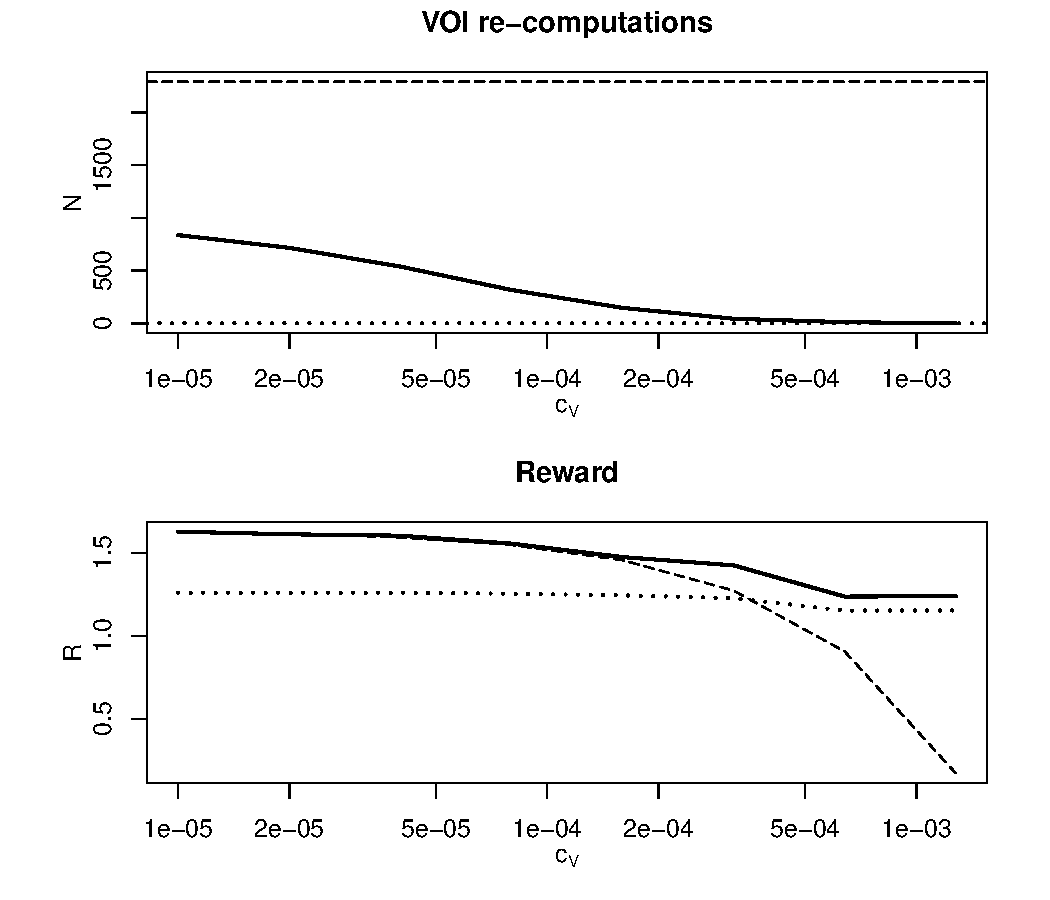
\includegraphics[scale=0.63]{raticomp-ackley.pdf}
\caption{The Ackley function.}
\label{fig:ackley}
\end{figure}
The Ackley function \cite{Ackley.function} is a popular optimization
benchmark. The two-argument form of the Ackley function is used in the
experiment; the function is defined by the expression (\ref{eq:emp-ackley}):
\begin{equation}
\label{eq:emp-ackley}
A(x,y)=20\cdot \exp\left(-0.2\sqrt { \frac {x^2+y^2} 2}\right)+\exp\left(\frac{cos(2\pi x)+cos(2\pi y)} 2\right)
\end{equation}
In the optimization problem, the utility function is
$u(z)=\tanh(2z)$, the measurements are normally distributed around the
true values with variance $\sigma_m^2=0.5$, and the measurement cost is
$0.01$. There are uniform dependencies with $\sigma_w^2=0.5$ in both
directions of the coordinate grid with a step of $0.2$ along each axis.
The results are presented in Figure~\ref{fig:ackley}.

\subsection{SVM Parameter Search}
\label{sec:raticomp-svm}

\begin{figure}[h]
\centering
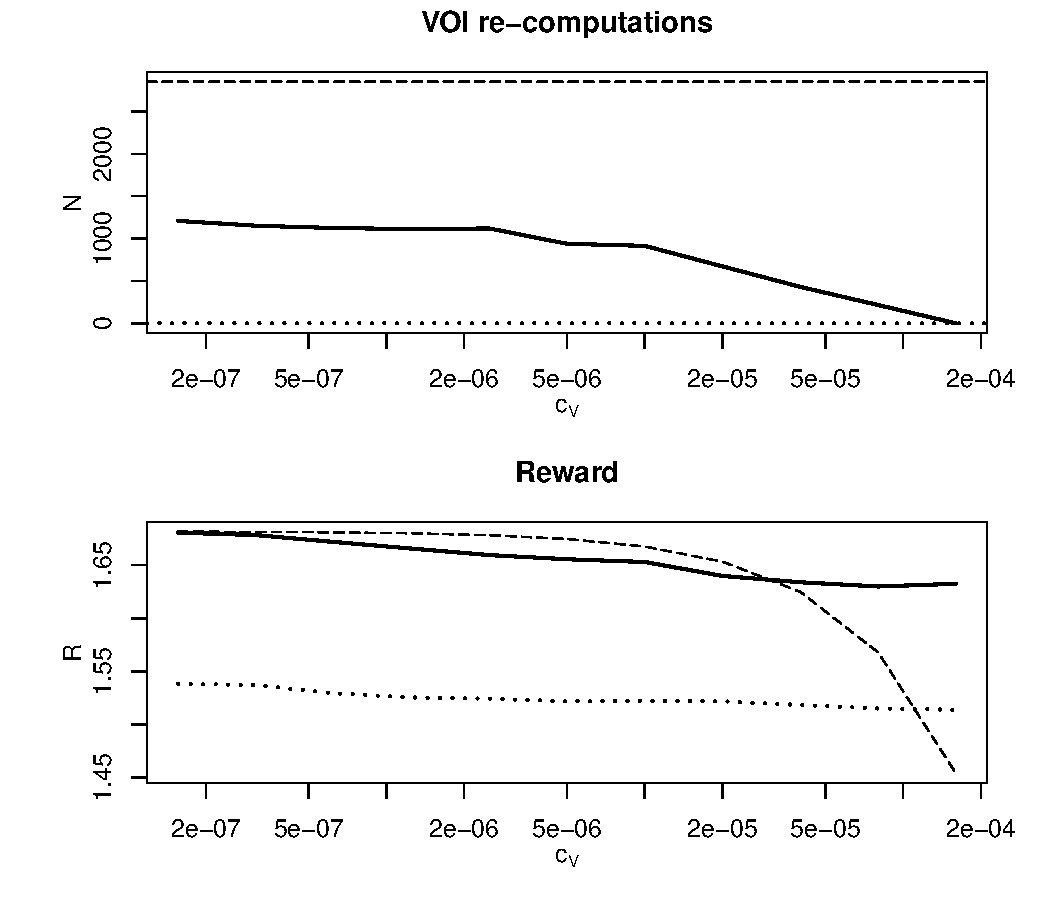
\includegraphics[scale=0.63]{raticomp-svmguide2.pdf}
\caption{SVM parameter search.}
\label{fig:svmguide2}
\end{figure}
An SVM (Support Vector Machine) classifier based on the radial basis
function has two parameters: $C$ and $\gamma$.  A combination of $C$
and $\gamma$ with high expected classification accuracy should be
chosen, and an efficient algorithm for determining the optimal values
is not known. A trial for a combination of parameters determines
estimated accuracy of the classifier through cross-validation. The
{\sc svmguide2} \cite{Hsu.dataset} dataset is used for the case study.
The utility function is $u(z)=\tanh(4(z-0.5))$, the $\log C$ and $\log
\gamma$ axes are scaled for uniformity to ranges $[1..21]$ and there
are uniform dependencies along both axes with $\sigma_w^2=0.4$. The
measurements are normally distributed with variance $\sigma_m^2=0.25$
around the true values, and the measurement cost is $c=0.01$.
The results are presented in Figure~\ref{fig:svmguide2}.

\subsection{Discussion of Results}

In all experiments, the reward, including the computation cost, of the
rational recomputing algorithm is comparable to or higher than the
reward of the original algorithm. When the computation cost is
relatively small (left-hand side of the plots), the rewards of the
rational recomputing algorithm and of the original algorithms are
essentially the same, despite the fact that much fewer VOI estimations are
computed. This suggests that the \textit{benefit of estimating the VOI}
of a measurement is in many cases low, and rational elective VOI
estimation is a viable approach to decreasing computation costs.
When the computation cost of VOI estimation grows, the rewards still
remain comparable, with the reward of the original algorithm only
slighter greater for the SVM parameter search
(Figure~\ref{fig:svmguide2}): a lower utility of the final choice of the
rational recomputing algorithm is compensated by a lower computation
cost. 

The advantage of the rational recomputing algorithm becomes obvious
when the cost of estimating the VOI of all measurements is comparable
to or exceeds the cost of performing a measurement (the right-hand side of
the plots). The reward of the original algorithm decreases rapidly,
falling below the reward of the Monte-Carlo algorithm. Rational
recomputing algorithm still performs well: the reward degrades
gradually with the increase of the computation cost, and approaches
asymptotically from above to the reward of random sampling (the
Monte-Carlo algorithm). 

Overall, the rational recomputing algorithm is robust, despite the
simplicity of the model. Both the case of a negligibly low computation
cost of VOI estimation, where both the original and the rational
recomputing algorithm exhibit good performance, and the case when the
cost of recomputation of VOI for all measurements is comparable to the
cost of performing a measurement are handled well: the reward is
almost as high as that of the original algorithm in the former case, and is
higher than that of Monte-Carlo algorithm performing the same number of
measurements in the latter case.

\section{Conclusion and Further Research}
\label{sec:raticomp-conclusion}

This chapter proposes an improvement to a widely used class of VOI-based
optimization algorithms. The improvement allows to decrease the
computation time while only slightly affecting the reward. The
proposed algorithm rationally reuses computations of VOI estimates and
recomputes the estimates only for measurements for which a change in
the VOI is likely to affect the choice of the next
measurement.

The proposed scheme of rational VOI computation can be further
improved. 
\begin{itemize}
\item  the normal distribution is chosen rather arbitrarily to model
  uncertainty about the VOI. Often, the VOI of a
  computational action decreases when other computational actions are  
  performed \cite{Guestrin.submodular}, and a skewed distribution from the
  exponential family should be chosen for better results.
\item The termination condition of VOI recomputation should be
  improved such that the VOI recomputation cost could be accounted for
  in the final reward.
\item The scheme is applied to the greedy algorithm
  for measurement selection, but can be extended to other
  VOI-based algorithms.
\end{itemize}


\chapter{Case Studies}
\label{ch:case-studies}

\section{Rational Deployment of CSP Heuristics}
\label{sec:cs-csp}
% $Id: thesis.tex,v 1.60 2010/04/13 11:12:30 dvd Exp $


\subsection{Introduction}

Large search spaces are common in artificial intelligence, heuristics being
of major importance in limiting search efforts.
The role of a heuristic, depending on type of search algorithm,
is to decrease the number of nodes expanded (e.g. in A* search),
the number of candidate actions considered (planning), or
the number of backtracks in constraint satisfaction problem (CSP) solvers.
Nevertheless, some sophisticated heuristics have considerable
computational overhead, significantly decreasing their overall effect
\cite{HorschHavens.pac,Kask.solcount},
even causing {\em increased} total runtime in pathological cases.
It has been recognized that control of this overhead can be essential
to improve search performance; e.g. by selecting which heuristics to evaluate
in a manner dependent on the state of the search \cite{Wallace.macheur,Domshlak.maxornot}.

We propose a rational metareasoning approach \cite{Russell.right} to decide
when and how to deploy heuristics, using CSP backtracking search as a case study.
The heuristics examined are various {\em solution count estimate} heuristics for
value ordering \cite{Meisels.solcount,HorschHavens.pac}, which
are expensive to compute, but can significantly decrease the number of
backtracks. These heuristics make a good case study, as their overall utility, taking computational
overhead into account, is sometimes detrimental; and yet,
by employing these heuristics adaptively, it may still be possible to achieve an
overall runtime improvement, even in these pathological cases.
Following the metareasoning approach, the value of information (VOI) of
a heuristic is defined in terms of total search time saved, and the
heuristic is computed such that the expected net VOI is positive.

We begin with background on metareasoning and CSP (Section~\ref{sec:csp-background}), 
followed by a re-statement of value ordering in terms
of rational metareasoning (Section~\ref{sec:csp-generic}), allowing a definition of VOI
of a value-ordering heuristics --- a contribution of this paper.
This scheme is then instantiated to handle
our case-study of backtracking search in CSP (Section~\ref{sec:csp-csp-rational}),
with parameters specific to value-ordering
heuristics based on solution-count estimates, the main contribution of this paper.
Empirical results (Section~\ref{sec:csp-empirical})
show that the proposed mechanism successfully balances the tradeoff
between decreasing backtracking and
heuristic computational overhead, resulting in a significant overall search time reduction.
Other aspects of such tradeoffs are also analyzed empirically.
Finally, related work is examined (Section~\ref{sec:csp-discussion}), and
possible future extensions of the proposed mechanism are discussed
(Section~\ref{sec:csp-summary}).


\subsection{Constraint Satisfaction}

A constraint satisfaction problem (CSP) is defined by a set
of variables $\mathcal{X}=\{X_1, X_2, ...\}$, and a set of
constraints $\mathcal{C}=\{C_1, C_2, ...\}$. Each variable $X_i$ has a non-empty domain
$D_i$ of possible values. Each constraint $C_i$ involves some subset
of the variables---the scope of the constraint--- and specifies the
allowable combinations of values for that subset. An assignment that
does not violate any constraints is called {\em consistent} (or {\em a solution}).
There are numerous variants of CSP settings and algorithmic paradigms. This
paper focuses on binary CSPs over discrete-values variables,
and backtracking search algorithms \cite{Tsang.csp}.

%A constraint satisfaction problem instance may or may not have a consistent
%assignment. 
%CSP search algorithm performance is
%determined by the computation time required to either find a
%solution or to prove that no solution exists.
A basic method used in numerous CSP search algorithm is
that of maintaining arc consistency (MAC)
\cite{Sabin.mac}. There are several versions of MAC; all
share the common notion of {\em
arc consistency}.
%, defined for CSP problems with binary constraints. 
A variable $X_i$ is arc-consistent with $X_j$ if for every value $a$ of
$X_i$ from the domain $D_i$ there is a value $b$ of $X_j$ from the
domain $D_j$ satisfying the constraint between $X_i$ and $X_j$. MAC
maintains arc consistency for all pairs of variables, and
speeds up backtracking search by pruning many inconsistent
branches.

CSP backtracking search algorithms typically employ
both variable-ordering \cite{Tsang.csp} and value-ordering heuristics.
The latter type include \emph{minimum conflicts} \cite{Tsang.csp}, which
orders values by the number of conflicts they cause
with unassigned variables, \emph{Geelen's promise}
\cite{Geelen.promise} --- by the product of domain sizes,
and \emph{minimum impact}
\cite{Refalo.impact} orders values by relative impact of the value
assignment on the product of the domain sizes.

Some value-ordering heuristics are based on solution count estimates
\cite{Meisels.solcount,HorschHavens.pac,Kask.solcount}: solution
counts for each value assignment of the current variable are
estimated, and assignments (branches) with the greatest solution count
are searched first.  The heuristics are based on the assumption that
the estimates are correlated with the true number of solutions, and
thus a greater solution count estimate means a higher probability that
a solution be found in a branch, as well as a shorter search time to
find the first solution if one exists in that
branch. \cite{Meisels.solcount} estimate solution counts by
approximating marginal probabilities in a Bayesian network derived
from the constraint graph; \cite{HorschHavens.pac} propose the
\emph{probabilistic arc consistency} heuristic (pAC) based on
iterative belief propagation for a better accuracy of relative
solution count estimates; \cite{Kask.solcount} adapt Iterative
Join-Graph Propagation to solution counting, allowing a tradeoff
between accuracy and complexity. These methods vary by computation
time and precision, although all are rather computationally
heavy. Principles of rational metareasoning can be applied
independently of the choice of implementation, to decide when
to deploy these heuristics.

\subsection{Rational Value-Ordering}
\label{sec:csp-generic}

The role of (dynamic) value ordering is to determine the order of
values to assign to a variable $X_k$ from its domain $D_k$, at a
search state where values have already been assigned to $(X_1, ...,
X_{k-1})$. We make the standard assumption that the ordering may
depend on the search state, but is not re-computed as a result of
backtracking from the initial value assignments to $X_k$: a new
ordering is considered only after backtracking up the search tree
above $X_k$.

Value ordering heuristics provide information on future search
efforts, which can be summarized by 2 parameters:
\begin{itemize}
\item  $T_i$---the expected time to find a solution containing
  assignment  $X_k=y_{ki}$ or verify that there are no such solutions;
\item  $p_i$---the ``backtracking probability'', that there will be no solution
consistent with $X_k=y_{ki}$.
\end{itemize}
These are treated as the algorithm's subjective probabilities about future search
in the current problem instance, rather than actual distributions over problem instances.
Assuming correct values of these parameters, and independence of backtracks,
the expected remaining search time in the subtree under $X_k$ for ordering $\omega$ is given by:
\begin{equation}
\label{eq:expected-search-time}
T^{s|\omega}=T_{\omega(1)}+\sum_{i=2}^{|D_k|}T_{\omega(i)}\prod_{j=1}^{i-1}p_{\omega(j)}
\end{equation}
In terms of rational metareasoning, the ``current'' optimal base-level action is picking
the $\omega $ which optimizes $T^{s|\omega}$.
Based on a general property of functions on sequences \cite{MonmaSidney.sequencing}, it can
be shown that $T^{s|\omega}$ is minimal if 
the values are sorted  by increasing order of $\frac {T_i} {1-p_i}$.

A candidate heuristic $H$ (with computation time $T^H$)  generates
an ordering by providing an updated (hopefully more precise)
value of the parameters $T_i, p_i$ for value assignments
$X_k=y_{ki}$, which may lead to a new optimal ordering $\omega_H$,
corresponding to a new base-level action.  The total expected
remaining search time is given by:

\begin{equation}
\label{eq:net-expected-time}
T=T^H+E[T^{s|\omega_H}]
\end{equation}

Since both $T^H$ (the ``time cost'' of $H$ in metareasoning terms)
and $T^{s|\omega_H}$ contribute to $T$, even a heuristic that
improves the estimates and ordering may not be useful.  It may be better not
to deploy $H$ at all, or to update $T_i, p_i$ only for some of the assignments.
According to the rational metareasoning approach (Section~\ref{sec:csp-ratimeta}),
the intrinsic VOI $\Lambda_i$ of estimating $T_i, p_i$ for the $i$th assignment
is the expected decrease in the expected search time:
\begin{equation}
\label{eq:value-ordering-benefit}
\Lambda_i=\IE\left[T^{s|\omega_-}-T^{s|\omega_{+i}}\right]
\end{equation}
where $\omega_-$ is the optimal ordering based on priors,
and $\omega_{+i}$ on values after updating $T_i, p_i$.
Computing new estimates (with overhead $T^c$) for values $T_i, p_i$
is beneficial just when the net VOI is positive:
\begin{equation}
\label{eq:voi}
V_i=\Lambda_i-T^c
\end{equation}
To simplify estimation of $\Lambda_i$, the expected
search time of an ordering is estimated as though the parameters are
computed only for $\omega_-(1)$, i.e. for the first value in the ordering;
essentially, this is the metareasoning subtree independence assumption.
 Other value assignments are assumed to have the prior (``default'')
parameters $T_\mathrm{def}, p_\mathrm{def}$. Assuming w.l.o.g. that $\omega_-(1)=1$:
\begin{equation}
\label{eq:time-estimate}
T^{s|\omega_-}=T_1+p_1\sum_{i=2}^{|D_k|}T_\mathrm{def}p_\mathrm{def}^{i-2}
   =T_1+p_1T_\mathrm{def}\frac{1-p_\mathrm{def}^{(|D_k|-1)}} {1-p_\mathrm{def}}
\end{equation}
and the intrinsic VOI of the $i$th deliberation action is:
\begin{equation}
\label{eq:benefit-estimate}
\Lambda_i=\IE\left[G(T_i, p_i)\,\Big|\;\frac {T_i} {1-p_i} < \frac {T_1} {1-p_1}\right]
\end{equation}
where $G(T_i, p_i)$ is the search time gain given the heuristically computed values $T_i, p_i$:
\begin{equation}
\label{eq:gain}
G(T_i, p_i) = T_1-T_i+(p_1-p_i)T_\mathrm{def}\frac{1-p_\mathrm{def}^{(|D_k|-1)}}{1-p_\mathrm{def}}
\end{equation}
In some cases, $H$ provides estimates only for the expected
search time $T_i$. In such cases, the backtracking probability $p_i$
can be bounded by the Markov inequality as the probability for the
given assignment that the time $t$ to find a solution or to verify that
no solution exists is at least the time $T_i^{all}$ to find all
solutions: $p_i=P\left(t\ge T_i^{all}\right)\le \frac{T_i} {T_i^{all}}$, 
and the bound can be used to estimate the probability:
\begin{equation}
\label{eq:backtracking-probability-estimate}
p_i\approx\frac{T_i} {T_i^{all}}
\end{equation}

Furthermore, note that in harder problems  the probability of
backtracking from variable $X_k$ is proportional to $p_\mathrm{def}^{(|D_k|-1)}$, and it is
reasonable to assume that backtracking probabilities above $X_k$
(trying values for $X_1, ..., X_{k-1}$)  are still significantly greater than 0.
Thus, the ``default'' backtracking
probability $p_\mathrm{def}$ is close to 1, and consequently:
\begin{equation}
  \label{eq:p-approx-one-estimate}
T_i^{all} \approx T_\mathrm{def},\quad\frac{1-p_\mathrm{def}^{(|D_k|-1)}}{1-p_\mathrm{def}} \approx |D_k|-1
\end{equation}
By substituting (\ref{eq:backtracking-probability-estimate}),
(\ref{eq:p-approx-one-estimate}) into (\ref{eq:gain}),
estimate (\ref{eq:gain-estimate}) for $G(T_i, p_i)$ is obtained:
\begin{eqnarray}
\label{eq:gain-estimate}
G(T_i, p_i)&\approx&T_1-T_i+(\frac {T_1} {T_1^{all}}-\frac {T_i} {T_i^{all}})T_\mathrm{def}\frac{1-p_\mathrm{def}^{(|D_k|-1)}}{1-p_\mathrm{def}}\nonumber\\
%           &\approx&T_1-T_i+(\frac {T_1} {T_\mathrm{def}}-\frac {T_i} {T_\mathrm{def}})T_\mathrm{def}\frac{1-p_\mathrm{def}^{(|D_k|-1)}}{1-p_\mathrm{def}}\nonumber\\
%           &\approx&T_1-T_i+(T_1-T_i)(|D_k|-1)\nonumber\\
           &\approx&(T_1-T_i)|D_k|
\end{eqnarray}
Finally, since (\ref{eq:backtracking-probability-estimate}), (\ref{eq:p-approx-one-estimate}) imply that $T_i<T_1 \Leftrightarrow \frac {T_i} {1-p_i} < \frac {T_1} {1-p_1}$, 
\begin{eqnarray}
\label{eq:benefit-superestimate}
\Lambda_i\approx\IE\left[(T_1-T_i)|D_k|\,\Big|\; T_i<T_1 \right]
\end{eqnarray}

\subsection{VOI of Solution Count Estimates}
\label{sec:csp-csp-rational}

The estimated solution count for an assignment may be used to estimate
the expected time to find a solution for the assignment under the
following assumptions\footnote{We do not claim
that this is a valid model of CSP search; rather, we argue that even with such a crude model
one can get significant runtime improvements.}:
\begin{enumerate}
\item Solutions are roughly evenly distributed in the search space, that is,
   the distribution of time to find a solution can be modeled by a
   Poisson process.
\item Finding all solutions for an assignment $X_{k}=y_{ki}$
takes roughly the same time for all assignments to the variable $X_k$. Prior work
   \cite{Meisels.solcount,Kask.solcount} demonstrates that
   ignoring the differences in subproblem sizes is justified.
\item The expected time to find all solutions for an assignment
  divided by its solution count estimate is a
  reasonable estimate for the expected time to find a single solution. 
\end{enumerate}
Based on these assumptions, $T_i$ can be estimated as $\frac {T^{all}}
{|D_k|n_i}$ where $T^{all}$ is the expected time to find all
solutions for all values of $X_k$, and $n_i$ is the
solution count estimate for $y_{ki}$; likewise, $T_1=\frac
{T^{all}} {|D_k|n_\mathrm{max}}$, where $n_\mathrm{max}$ is the currently
greatest $n_i$.  By substituting the expressions for
$T_i$, $T_1$ into (\ref{eq:benefit-superestimate}), obtain
%(\ref{eq:benefit-estimate-sc}) 
as the intrinsic VOI of computing $n_i$:
\begin{equation}
\label{eq:benefit-estimate-sc}
\Lambda_i=T^{all} \sum_{n=n_\mathrm{max}}^\infty\left(
  \frac 1 {n_\mathrm{max}} - \frac 1 n\right) P(n, \nu)
\end{equation}
where $P(n, \nu)=e^{-\nu}\frac {\nu^n} {n!}$ is the probability,
according to the Poisson distribution, to find $n$ solutions for a
particular assignment when the mean number of solutions per assignment
is $\nu=\frac N {|D_k|}$, and $N$ is the estimated solution count for
all values of $X_k$, computed at an earlier stage of the algorithm.

Neither $T^{all}$ nor $T^c$, the time to estimate the solution count
for an assignment, are known. However, for relatively low solution
counts, when an invocation of the heuristic has high intrinsic VOI, both
$T^{all}$ and $T^c$ are mostly determined by the time spent eliminating
non-solutions. Therefore, $T^c$ can be assumed approximately proportional
to $\frac {T^{all}} {|D_k|}$, the average time to find all solutions
for a single assignment, with an unknown factor $\gamma < 1$:

\begin{equation}
\label{eq:csp-gamma}
T^c \approx \gamma \frac {T^{all}} {|D_k|}
\end{equation}
Then, $T^{all}$ can be eliminated from both $T^c$ and $\Lambda$. 
Following Equation~(\ref{eq:voi}), the solution count 
should be estimated whenever the net VOI is positive:
\begin{equation}
\label{eq:csp-solcount-condition}
V(n_\mathrm{max}) \propto |D_k|e^{-\nu}\sum_{n=n_\mathrm{max}}^\infty \! \! \left( \frac 1 {n_\mathrm{max}} - \frac 1 n\right) \frac {\nu^n} {n!}-\gamma
\end{equation}
The infinite series in
(\ref{eq:csp-solcount-condition}) rapidly converges, and an
approximation of the sum can be computed efficiently. As done
in Section \ref{sec:csp-empirical}, $\gamma$ can be learned
offline from a set of problem instances of a certain kind for the
given implementation of the search algorithm and the solution counting
heuristic.

Algorithm~\ref{alg:csp-solcount} implements rational value ordering.
The procedure receives problem instance $csp$ with assigned values for
variables $X_1, ..., X_{k-1}$, variable $X_k$ to be ordered, and
estimate $N$ of the number of solutions of the problem instance
(line~\ref{alg:csp-solcount-args}); $N$ is computed at the previous
step of the backtracking algorithm as the solution count estimate for
the chosen assignment for $X_{k-1}$, or, if $k=1$, at the beginning of
the search as the total solution count estimate for the
instance. Solution counts $n_i$ for some of the assignments are
estimated (lines~\ref{alg:csp-solcount-while}--\ref{alg:csp-solcount-endwhile})
by selectively invoking the heuristic computation {\sc
  EstimateSolutionCount} (line~\ref{alg:csp-estimate-solution-count}),
and then the domain of $X_k$, ordered by non-increasing solution count
estimates of value assignments, is returned
(lines~\ref{alg:csp-solcount-sort}--\ref{alg:csp-solcount-return}).

\begin{algorithm}[h]
\caption{Value Ordering via Solution Count Estimation}
\label{alg:csp-solcount}
\begin{algorithmic}[1]
\Procedure{ValueOrdering-SC}{$csp, X_k, N$}\label{alg:csp-solcount-args}
  \State $D \gets D_k$,\hspace{1em}$n_\mathrm{max} \gets \frac N {|D|}$
  \State {\bf for all} {$i$ {\bf in} $1..|D|$} {\bf do} $n_i \gets n_\mathrm{max}$
  \While {$V(n_\mathrm{max})>0$} \label{alg:csp-solcount-while} \Comment using Equation~(\ref{eq:csp-solcount-condition})
    \State choose $y_{ki} \in D$ arbitrarily
    \State $D \gets D \setminus \{y_{ki}\}$
    \State $csp' \gets csp$ with $D_k=\{y_{ki}\}$
    \State $n_i \gets$ {\sc EstimateSolutionCount}($csp'$) \label{alg:csp-estimate-solution-count}
    \State {\bf if} {$n_i>n_\mathrm{max}$} {\bf then} $n_\mathrm{max} \gets n_i$
  \EndWhile \label{alg:csp-solcount-endwhile}
  \State {\bf end while}
  \State $D_{ord} \gets$ sort $D_k$ by non-increasing $n_i$ \label{alg:csp-solcount-sort}
  \State {\bf return} $D_{ord}$ \label{alg:csp-solcount-return}
\EndProcedure
\end{algorithmic}
\end{algorithm}

\subsection{Empirical Evaluation}
\label{sec:csp-empirical}

%The dependence of the searchm time on $\gamma$
%(\ref{eq:csp-solcount-condition}) over a range of constraint satisfaction
%problems must be explored empirically. 

Specifying the algorithm parameter $\gamma$ is the first issue.
$\gamma$ should be a characteristic of the
implementation of the search algorithm, rather than of the problem
instance; it is also desirable that the performance of the algorithm not
be too sensitive to fine tuning of this parameter.

%varying the number of assignments for which the
%solution count is estimated based on Equation (\ref{eq:csp-solcount-condition}).

Most of the  experiments were conducted on sets of random problem instances
generated according to Model RB \cite{Xu.rb}. The empirical evaluation
was performed in two stages. In the first stage, several benchmarks
were solved for a wide range of values of $\gamma$, and an appropriate
value for $\gamma$ was chosen. In the second stage, the search was run
on two sets of problem instances with the chosen $\gamma$, as well as
with exhaustive deployment, and with the minimum conflicts
heuristic, and the search time distributions were compared for each of
the value-ordering heuristics.

The AC-3 version of MAC was used for the experiments, with some
modifications \cite{Sabin.mac}. Variables were ordered using the
maximum degree variable ordering heuristic.\footnote{A dynamic
variable ordering heuristic, such as dom/deg, may result in shorter
search times in general, but gave no significant improvement in our
experiments; on the other hand, static variable ordering simplifies
the analysis.} The value-ordering heuristic was based on a version
of the solution count estimate proposed in \cite{Meisels.solcount}.
The version used in this paper was optimized for better computation
time for overconstrained problem instances. As a result,
Equation~(\ref{eq:csp-gamma}) is a reasonable
approximation for this implementation. The source code is available from
\url{http://ftp.davidashen.net/vsc.tar.gz}.

\subsubsection{Benchmarks}

\begin{figure}[h]
\centering
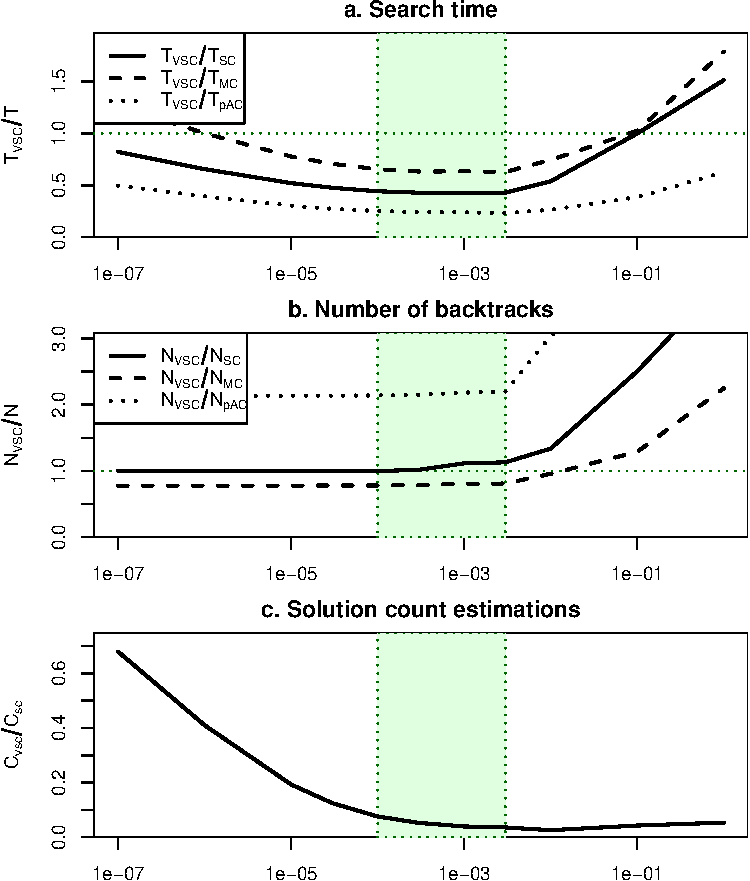
\includegraphics[scale=0.75]{csp-benchmarks.pdf}
\caption{Influence of $\gamma$ in CSP benchmarks}
\label{fig:benchmarks}
\end{figure}

CSP benchmarks from CSP Solver Competition~2005
\cite{Boussemart.benchmarks} were used. 14 out of 26 benchmarks
solved by at least one of the solvers submitted for the competition
could be solved with 30 minutes timeout by the solver used for this
empirical study for all values of $\gamma$: $\gamma=0$ and the
exponential range $\gamma \in \{10^{-7}, 10^{-6}, ..., 1\}$, as well
as with the minimum-conflicts heuristic and the pAC heuristic.

Figure~\ref{fig:benchmarks}.a shows the mean search time of VOI-driven
solution count estimate deployment $T_{VSC}$ normalized by the search
time of exhaustive deployment $T_{SC}$ ($\gamma=0$), for the minimum
conflicts heuristic $T_{MC}$, and for the pAC heuristic $T_{PAC}$.
The shortest search time on average is achieved by VSC for $\gamma \in
[10^{-4},3\cdot10^{-3}]$ (shaded in the figure) and is much shorter
than for SC ($\mean \left(\frac {T_{VSC}(10^{-3})}
{T_{SC}}\right)\approx 0.45$); the improvement was
  actually close to the ``ideal'' of getting all the information
  provided by the heuristic without paying the overhead at all. For
all but one of the 14 benchmarks the search time for VSC with
$\gamma=3\cdot10^{-3}$ is shorter than for MC. For most values of
$\gamma$, VSC gives better results than MC ($\frac {T_{VSC}} {T_{MC}}
< 1$). pAC always results in the longest search time due to the
computational overhead.

Figure~\ref{fig:benchmarks}.b shows the mean number of backtracks of
VOI-driven deployment $N_{VSC}$ normalized by the
number of backtracks of exhaustive deployment $N_{SC}$,
the minimum conflicts heuristic $N_{MC}$, and for
the pAC heuristic $\overline N_{pAC}$. VSC causes less backtracking
than MC for $\gamma\le 3\cdot10^{-3}$ ($\frac {N_{VSC}}  {N_{MC}} <
1$). pAC always causes less backtracking than other heuristics, but
has overwhelming computational overhead.

Figure~\ref{fig:benchmarks}.c shows $C_{VSC}$, the number of
estimated solution counts of VOI-driven deployment, normalized by the
number of estimated solution counts of exhaustive deployment
$C_{SC}$. When $\gamma=10^{-3}$ and the best search time is achieved,
the solution counts are estimated  only in a relatively small number
of search states: the average number of estimations is ten times smaller than in the
exhaustive case ($\mean\left(\frac {C_{VSC}(10^{-3})}
{C_{SC}}\right)\approx 0.099$, $\median\left(\frac {C_{VSC}(10^{-3})}
{C_{SC}}\right)\approx 0.048$). 

The results show that although the solution counting heuristic
may provide significant improvement in the search time, further improvement is
achieved when the solution count is estimated only in a \emph{small fraction of
occasions} selected using rational metareasoning.

\begin{figure}[h] 
\centering
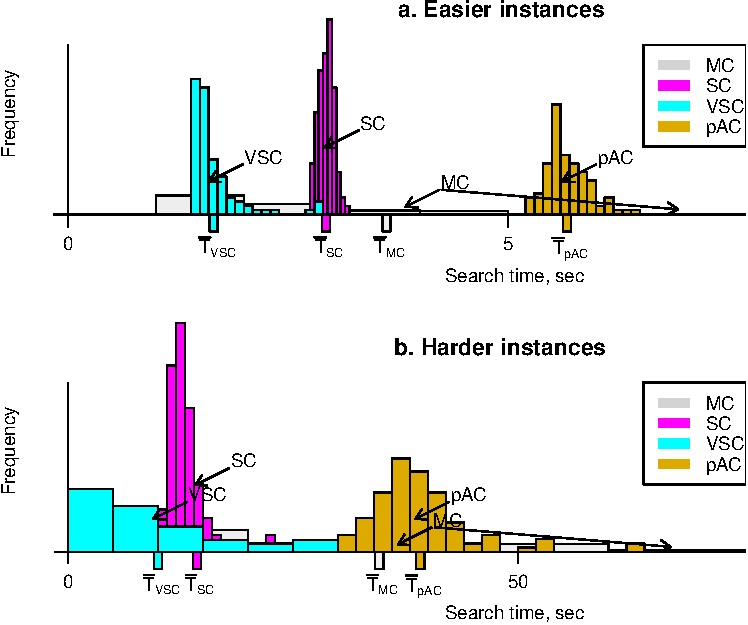
\includegraphics[scale=0.75]{csp-random-problems-arrows+legend.pdf}
\caption{Search time comparison on sets of random instances (using
  Model RB)}
\label{fig:random-problems}
\end{figure}

\subsubsection{Random instances}

Based on the results on benchmarks, we chose $\gamma=10^{-3}$, and
applied it to two sets of 100 problem instances. 
Exhaustive deployment, rational deployment, the
minimum conflicts heuristic, and probabilistic arc consistency
were compared.

The first, easier, set was generated with 30 variables, 30 values per
domain, 280 constraints, and 220 nogood pairs per constraint
($p=0.24,\;p_{crit}=0.30$). Search time distributions are presented in
Figure~\ref{fig:random-problems}.a. The shortest mean search time is
achieved for rational deployment, with exhaustive deployment
next ($\frac {\overline T_{SC}} {\overline T_{VSC}}
\approx 1.75 $), followed by the minimum conflicts heuristic ($\frac
{\overline T_{MC}} {\overline T_{VSC}} \approx 2.16$) and 
probabilistic arc consistency ($\frac {\overline T_{pAC}} {\overline
  T_{VSC}} \approx 3.42$). Additionally,
while the search time distributions for solution counting are sharp
($\frac {\max T_{SC}} {\overline T_{SC}} \approx 1.08$, $\frac {\max
T_{VSC}} {\overline T_{VSC}} \approx 1.73$), the distribution for the
minimum conflicts heuristic has a long tail with a much longer worst
case time ($\frac {\max T_{VSC}} {\overline T_{VSC}} \approx 5.67$).

The second, harder, set was generated with 40 variables, 19 values,
410 constraints, 90 nogood pairs per constraint (exactly at the phase
transition: $p=p_{crit}=0.25$).
Search time distributions are presented in Figure~\ref{fig:random-problems}.b.
As with the first set, the shortest mean search time is achieved for
rational deployment: $\frac {\overline T_{SC}} {\overline T_{VSC}}
\approx 1.43 $,  while the relative mean search time for the minimum
conflicts heuristic is much longer: $\frac {\overline T_{MC}}
{\overline T_{VSC}} \approx 3.45$. The probabilistic arc consistency heuristic
resulted again in the longest search time due to the overhead of computing
relative solution count estimates by loopy belief propagation: $\frac
{\max T_{VSC}} {\overline T_{VSC}} \approx 3.91$. 

Thus, the value of $\gamma$ chosen based on a small set of hard instances
gives good results on a set of instances with different parameters and
of varying hardness.

\subsubsection{Generalized Sudoku}

Randomly generated problem instances have played a key role in the
design and study of heuristics for CSP. However, one might argue that the
benefits of our scheme are specific to model RB. Indeed, real-world problem
instances often have much more structure than random instances
generated according to Model RB. Hence, we repeated the experiments
on randomly generated Generalized Sudoku
instances \cite{Ansotegui.sudoku}, since this domain is highly
structured, and thus a better source of realistic problems with a controlled
measure of hardness.

%and relative performance of various heuristics on these
%instances can be significantly different compared to unstructured
%random instances.

The search was run on two sets of 100 Generalized Sudoku instances,
with 4x3 tiles and 90 holes and with 7x4 tiles and 357 holes, with
holes punched using the doubly balanced method
\cite{Ansotegui.sudoku}. The search was repeated on each instance with
the exhaustive solution-counting, VOI-driven solution counting (with
the same value of $\gamma=10^{-3}$ as for the RB model problems),
minimum conflicts, and probabilistic arc
consistency value ordering heuristics. Results
are summarized in Table~\ref{tbl:sudoku} and show that relative
performance of the methods on Generalized Sudoku is similar to the
performance on Model RB.
\begin{table}[h]
\begin{center}
\small
\begin{tabular}{r|c|c|c|c}
               & $\overline {T_{SC}}$, sec & $\overline {\left(\frac
                   {T_{VSC}} {T_{SC}}\right)}$ & $\overline
               {\left(\frac {T_{MC}} {T_{SC}}\right)}$ & $\overline
               {\left(\frac {T_{pAC}} {T_{SC}} \right)}$ \\  \hline
4x3, 90 holes &  1.809 & 0.755 & 1.278 & 22.421 \\  \hline
7x4, 357 holes & 21.328 & 0.868 & 3.889 & 3.826
\end{tabular}
\end{center}
\caption{Generalized Sudoku}
\label{tbl:sudoku}
\end{table}

\subsubsection{Deployment patterns}

One might ask whether trivial methods for selective deployment would
work, such as estimating solution counts for a certain number of
assignments in the beginning of the search. We examined deployment
patterns of VOI-driven SC with ($\gamma=10^{-3}$) on several instances
of different hardness. For all instances, the solution counts were
estimated at varying rates during \emph{all stages} of the search, and
the deployment patterns differed between the instances, so a simple
deployment scheme seems unlikely.

VOI-driven deployment also compares favorably to
random deployment. Table~\ref{tbl:voirnd} shows
performance of VOI-driven deployment for $\gamma=10^{-3}$ and of
uniform random deployment, with total number of solution count estimations
equal to that of the VOI-driven deployment.
For both schemes, the values for which solution
counts were not estimated were ordered randomly, and the search
was repeated 20 times.  The mean search time for the random deployment is
$\approx1.6$ times longer than for the VOI-driven deployment, and has
$\approx100$ times greater standard deviation.
\begin{table}[h]
\begin{center}
\small
\begin{tabular}{r|c|c|c}
               & $\mathrm{mean}(T)$, sec & $\mathrm{median}(T)$, sec & $\mathrm{sd}(T)$, sec \\ \hline
VOI-driven     & 19.841                  & 19.815                    & 0.188 \\ \hline
random         & 31.421                  & 42.085                    & 20.038  
\end{tabular}
\end{center}
\caption{VOI-driven vs. random deployment}
\label{tbl:voirnd}
\end{table}

\subsection{Discussion and Related Work}
\label{sec:csp-discussion}

The principles of bounded rationality appear in
\cite{Horvitz.reasoningabout}. \cite{Russell.right}
provided a formal description of rational metareasoning and case
studies of applications in several problem domains.
A typical use of rational metareasoning in search is in finding which node
to expand, or in a CSP context determining a variable or value assignment.
The approach taken in this paper adapts these methods to
whether to spend the time to compute a heuristic.

Runtime selection of heuristics has lately been of interest, e.g.
deploying heuristics for planning \cite{Domshlak.maxornot}. The approach
taken is usually that of {\em learning} which heuristics to deploy based on
features of the search state. Although our approach can also benefit from learning,
since we have a parameter that needs to be
tuned, its value is mostly algorithm dependent,
rather than problem-instance dependent. This simplifies learning 
considerably, as opposed to having to learn a classifier from scratch.
Comparing metareasoning techniques to learning techniques (or possibly a combination
of both, e.g. by learning more precise distribution models) is an interesting issue for future research.

Although rational metareasoning is applicable 
to other types of heuristics, solution-count estimation heuristics are
natural candidates for the type of optimization suggested in this paper.
\cite{Dechter.cspheur} first suggested solution
count estimates as a value-ordering heuristic (using propagation on trees)
for constraint satisfaction problems, refined in \cite{Meisels.solcount} to multi-path propagation.

\cite{HorschHavens.pac} used a value-ordering heuristic that estimated
relative solution counts to solve constraint satisfaction problems and
demonstrated efficiency of their algorithm (called pAC, probabilistic
Arc Consistency). However, the computational overhead of the heuristic was large,
and the relative solution counts were
computed offline. \cite{Kask.solcount} introduced a CSP algorithm
with a solution counting heuristic based on the Iterative Join-Graph Propagation
(IJGP-SC), and empirically showed performance advances over MAC in most cases.
In several cases IJGP-SC was still slower than MAC due to the computational
overhead. \cite{Kask.solcount} also used the IJGP-SC heuristic as the
value ordering heuristic for MAC.

Impact-based value ordering
\cite{Refalo.impact} is another heavy informative heuristic.  
One way to decrease its overhead, suggested in
\cite{Refalo.impact}, is to learn the impact of an assignment by averaging the impact of
earlier assignments of the same value to the same
variable. Rational deployment of this heuristic by estimating the probability 
of backtracking based on the impact may be possible, an issue for future research.
\cite{Gomes.solcount} propose a technique that adds random generalized XOR
constraints and counts solutions with high precision, but at present requires {\em solving} CSPs,
thus seems not to be immediately applicable as a search heuristic.

The work presented in this paper differs from the above related
schemes in that it does not attempt to introduce new heuristics
or solution-count estimates. Rather, an ``off the shelf''
heuristic is deployed selectively based on value of information,
thereby significantly reducing the heuristic's ``effective''
computational overhead, with an improvement in 
performance for problems of different size and hardness.

\subsection{Summary and Future Research}
\label{sec:csp-summary}

This paper suggests a model for adaptive deployment of value ordering
heuristics in algorithms for constraint satisfaction problems. As a
case study, the model was applied to a value-ordering heuristic based
on solution count estimates, and a steady improvement in the overall
algorithm performance was achieved compared to {\em always} computing
the estimates, as well as to other simple deployment tactics.  The
experiments showed that for many problem instances the optimum
performance is achieved when solution counts are estimated only in a
relatively small number of search states.

The methods introduced in this paper can be extended in numerous
ways. First, generalization of the VOI to deploy different types of
heuristics for CSP, such as variable ordering heuristics, as well as
reasoning about deployment of more than one heuristic at a time, are
natural non-trivial extensions. Second, an explicit evaluation of the
quality of the distribution model is an interesting issue, coupled
with a better candidate model of the distribution.  Such distribution
models can also employ more disciplined statistical learning methods
in tandem, as suggested above. Finally, applying the methods suggested
in this paper to search in other domains can be attempted, especially
to heuristics for planning.  In particular, examining whether
the meta-reasoning scheme can improve reasoning over deployment of
heuristics based solely on learning methods is an interesting future
research issue.



\clearpage
\section{VOI-aware Monte-Carlo Tree Search}
\label{sec:cs-mcts}

Monte Carlo Tree Search (MCTS), and especially UCT \cite{Kocsis.uct}
appears in numerous search applications, such
as \cite{Eyerich.ctp}. Although these methods are shown to be
successful empirically, most authors appear to be using UCT ``because
it has been shown to be successful in the past'', and ``because it
does a good job of trading off exploration and exploitation''. While
the latter statement may be correct for the Multi-armed Bandit problem (MAB)
and for the UCB1 algorithm \cite{Auer.ucb}, we argue that a simple
reconsideration from basic principles can result in schemes that
outperform UCT.

The core issue is that in MCTS for adversarial search and search in
``games against nature'' the goal is typically to find the best
first action of a good (or even optimal) policy, which is closer to
minimizing the simple regret, rather than the cumulative regret
minimized by UCB1.  However, the simple and the cumulative regret
cannot be minimized simultaneously; moreover, \cite{Bubeck.pure} shows
that in many cases the smaller the cumulative regret, the greater the
simple regret.

We begin with background definitions and related work.  VOI estimates
for arm pulls in MAB are presented, and a VOI-aware sampling policy is
suggested, both for the simple regret in MAB and for MCTS.  Finally,
the performance of the proposed sampling policy is evaluated on sets
of Bernoulli arms and on Computer GO, showing the improved
performance.

\section{Background and Related Work}
\label{sec:mcts-related-work}

Monte-Carlo tree search was initially suggested as a scheme for
finding approximately optimal policies for Markov Decision Processes
(MDP).  MCTS explores an MDP by performing
\emph{rollouts}---trajectories from the current state to a state in
which a termination condition is satisfied (either the goal or a
cutoff state).

Taking a sequence of samples in order to minimize the regret of a
decision based on the samples is captured by the Multi-armed Bandit
problem (MAB) \cite{Vermorel.bandits}. In MAB, we have a set of $K$
arms. Each arm can be pulled multiple times. When the $i$th arm is
pulled, a random reward $X_i$ from an unknown stationary distribution
is encountered. In the \textit{cumulative setting}, all encountered rewards are
collected.  UCB1 \cite{Auer.ucb} was shown to be
near-optimal in this respect. UCT, an extension of UCB1 to MCTS is
described in \cite{Kocsis.uct}, and shown to outperform many state of
the art search algorithms in both MDP and adversarial search
\cite{Gelly.mogo,Eyerich.ctp}. In the \textit{simple regret setting}, the agent
gets to collect only the reward of the last pull.
\begin{dfn}
The \textbf{simple regret} of a sampling policy for MAB
is the expected difference between the best expected reward
$\mu_*$ and the expected reward $\mu_j$ of the empirically best arm
$\overline X_j=\max_i\overline X_i$:
\begin{equation}
\IE r=\sum_{j=1}^K\Delta_j\Pr(\overline X_j=\max_i\overline X_i)
\label{eqn:mcts-simple-regret}
\end{equation}
where $\Delta_j=\mu_*-\mu_j$.
\end{dfn}
Strategies that minimize the simple regret are called pure exploration
strategies \cite{Bubeck.pure}. 

A different scheme for control of sampling can use the principles of 
rational metareasoning (Section~\ref{sec:ratimeta}).
In particular, a pure exploration strategy  based on the principles of
rational metareasoning would always select a sample with the highest
value of information, and stop the sampling when the VOI of the sample
is lower than the cost.

\section{Upper bounds on Value of Information}
\label{sec:mcts-approx-nonbayesian-section}

In many practical applications of the selection problem, such as search in
the game of Go, prior distributions are unavailable.\footnote{The analysis is also applicable to
some Bayesian settings, using ``fake" samples to simulate prior distributions.}
In such cases, one can still bound
the value of information of myopic policies using {\em concentration
inequalities} to derive distribution-independent bounds on the
VOI. We obtain such bounds under the
following assumptions:
\begin{enumerate}
\item Samples are iid given the value of the arms (variables), as in the Bayesian schemes such as Bernoulli
sampling.
\item The expectation of a selection in a belief state is equal to the sample mean (and therefore,
   after sampling terminates, the arm with the greatest sample mean will be selected).
\end{enumerate}

When considering possible samples in the blinkered semi-myopic setting,
two cases are possible: either
	the arm $\alpha$ with the highest sample mean $\overline
  	X_\alpha$ is tested, and $\overline X_\alpha$ becomes lower than
 	$\overline X_\beta$ of the second-best arm $\beta$;
or, 
	another arm~$i$ is tested, and $\overline X_i$ becomes higher
    than $\overline X_\alpha$.


Our bounds below are applicable to any bounded distribution (without loss of generality 
bounded in $[0,1]$). Similar
bounds can be derived for certain unbounded distributions, such as the
normally distributed prior value with normally distributed
sampling.
We derive a VOI bound for testing an arm a fixed $N$ times,
where $N$ can be the remaining budget of available samples or
any other integer quantity.
Denote by  $\Lambda_i^b$ the intrinsic VOI of testing the $i$th arm
$N$ times, the number of
samples already taken from the $i$th arm by $n_i$, \chg{and the sample mean
of $m$ outcomes from the $i$th arm by $X_i^m$, for any $m$.}
\begin{thm} $\Lambda_i^b$ is bounded from above as
\begin{align}
\label{eqn:mcts-thm-be}
\Lambda_{i|i\ne\alpha}^b&\le \frac {N(1-\overline X_\alpha^{n_\alpha})} {n_i}\Pr(\overline   X_i^{{n_i}+N}\ge\overline X_\alpha^{n_\alpha})\nonumber\\
\Lambda_\alpha^b&\le \frac {N \overline X_\beta^{n_\beta}} {n_\alpha} \Pr(\overline X_\alpha^{n_\alpha+N}\le\overline X_\beta^{n_\beta})
\end{align}
\label{thm:mcts-be}
\end{thm}
\begin{proof} For the case $i\ne \alpha$, the probability that the
	  $i$th arm is finally chosen instead of $\alpha$ is
	  $\Pr(\overline X_i^{n_i+N} \ge \overline X_\alpha^{n_\alpha})$. $X_i \le 1$,
	  therefore $\overline X_i^{n_i+N}\le \overline
	  X_\alpha^{n_\alpha}+\frac {N(1-\overline X_\alpha^{n_\alpha})} {N+n_i}$. Hence, the intrinsic value of blinkered
	  information is at most: 
	\begin{align}
	\label{eq:simplistic}
	\frac{ N(1-\overline  X_\alpha^{n_\alpha})}
	  {N+n_i}&\Pr(\overline X_i^{{n_i}+N}\ge\overline X_\alpha^{n_\alpha})\nonumber \\
	&\le\frac{ N(1-\overline  X_\alpha^{n_\alpha})}
	{n_i}\Pr(\overline X_i^{{n_i}+N}\ge\overline X_\alpha^{n_\alpha})
	\end{align}
	  Proof for the case $i=\alpha$ is similar.
\end{proof}


The probabilities can be bounded from above using the
Hoeffding inequality \cite{Hoeffding.ineq}:
\begin{thm} For any $A\ge\overline X_{i|i\ne\alpha}^{n_i}$ and $B\le\overline X_\alpha^{n_\alpha}$ the probabilities $\Pr(\overline X_{i|i\ne\alpha}^{n_i+N} \ge A)$, $\Pr(\overline X_\alpha^{{n_\alpha}+N} \le B)$ are bounded from above as
\begin{align}
  \label{eqn:mcts-probound-blnk-hoeffding}
  \Pr&(\overline X_{i|i\ne\alpha}^{n_i+N} \ge A) \le 2\exp\left(- \varphi (A -\overline  X_i^{n_i})^2 n_i \right)\nonumber\\
  \Pr&(\overline X_\alpha^{{n_\alpha}+N} \le B) \le 2\exp\left(- \varphi (\overline X_\alpha^{n_\alpha} - B)^2 n_\alpha\right)
\end{align}
where $\varphi=\min \left(2(\frac {1+n/N} {1+\sqrt {n/N}})^2\right)=8(\sqrt 2 - 1)^2 > 1.37$.
\label{thm:mcts-hoeffding-prob-bounds}
\end{thm}


\begin{proof}
	Equation~(\ref{eqn:mcts-probound-blnk-hoeffding}) follows from
        the observation that $\overline X_i^{n_i+N}>A$ if and only if
        the mean $\overline X_i^N$ of $N$ samples from $n_i+1$ to
        $n_i+N$ is at least $A+(A-\overline X_i^{n_i})\frac {n_i} N$.

	For any $\delta$, the probability that $\overline X_i^{n_i+N}$ is greater
	than $A$ is less than the probability that
	$\IE[X_i]\ge\overline X_i^n+\delta$
	\emph{or} $\overline X_i^N\ge \IE[X_i]+A -\overline X_i^{n_i} - \delta +(A - \overline X_i^{n_i})\frac {n_i} N$,
	thus, by the union bound, less than the sum of the probabilities:
	\begin{align}
	\Pr&(\overline X_i^{n_i+N}\ge A)\nonumber\\
	   &\le\Pr(\IE[X_i]-\overline X_i^{n_i} \ge \delta)\\
	   &+\Pr\left(\overline X_i^N - \IE[X_i] \ge A
	           - \overline X_i^{n_i} - \delta +(A - \overline X_i^{n_i})\frac {n_i} N\right)\nonumber
	\end{align}
	Bounding the probabilities on the right-hand side using the Hoeffding
	inequality, obtain:
	\begin{align}
	\Pr&(\overline X_i^{n_i+N}\ge A)\nonumber\\
	    &\le\exp(-2\delta^2n_i)\nonumber\\
	    &+\exp\left(-2\left((A - \overline X_i^{n_i})\left(1+\frac {n_i} N\right)-\delta\right)^2N\right)
	\label{eqn:mcts-app-hoeffding-le-maxexp}
	\end{align}
	Find $\delta$ for which the two terms on the right-hand side of
	Equation~(\ref{eqn:mcts-app-hoeffding-le-maxexp}) are equal:
	\begin{equation}
	\exp(-\delta^2n) = \exp\left(-2\left((A - \overline X_i^{n_i})(1+\frac {n_i} N) - \delta\right)^2N\right)\label{eqn:mcts-app-hoeffding-eq-exp}
	\end{equation}
	Solve Equation~(\ref{eqn:mcts-app-hoeffding-eq-exp}) for $\delta$: $\delta=\frac {1+\frac {n_i} N} {1+\sqrt {\frac {n_i} N}} (A - \overline X_i^{n_i}) \ge 2(\sqrt 2 - 1)(A-\overline X_i^{n_i})$. Substitute $\delta$ into 
	Equation~(\ref{eqn:mcts-app-hoeffding-le-maxexp}) and obtain
	\begin{align}
	\Pr&(\overline X_i^{n_i+N}\ge A) \nonumber\\
	& \le 2\exp\left(-2\left( \frac {1+\frac {n_i} N} {1+\sqrt {\frac {n_i} N}}
	                          (\overline X_\alpha^{n_\alpha} - \overline X_i^{n_i})\right)^2 n_i\right)\nonumber \\
	& \le 2\exp(-8(\sqrt 2 - 1)^2(A - \overline X_i^{n_i})^2n_i)\nonumber\\
	& = 2\exp(-\varphi(A - \overline X_i^{n_i})^2n_i)
	\end{align}
	Derivation for the case $i=\alpha$ is similar.
\end{proof}	

\begin{crl}
An upper bound on the VOI estimate $\Lambda_i^b$ is obtained
by substituting Equation~(\ref{eqn:mcts-probound-blnk-hoeffding}) into (\ref{eqn:mcts-thm-be}).
\begin{align}
  \label{eqn:mcts-bound-blnk-hoeffding}
  \Lambda&_{i|i\ne\alpha}^b\le \hat\Lambda_i^b=  \frac {2N(1-\overline  X_\alpha^{n_\alpha})} {n_i}\exp\left(- \varphi(\overline X_\alpha^{n_\alpha} - \overline X_i^{n_i})^2 n_i\right)\\
  \Lambda&_\alpha^b \le \hat\Lambda_\alpha^b=\frac {2N\overline X_\beta^{n_\beta}} {n_\alpha}\exp\left(- \varphi(\overline X_\alpha^{n_\alpha} - \overline X_\beta^{n_\beta})^2 n_\alpha\right)\nonumber
\end{align}
\label{crl:bound-blnk-hoeffding}
\end{crl}

More refined bounds can be obtained through tighter estimates on the
probabilities in Equation~(\ref{eqn:mcts-thm-be}), for example, based on the empirical Bernstein
inequality~\cite{MaurerPontil.benrstein}, or through a more careful
application of the Hoeffding inequality, resulting in Theorem~\ref{thm:mcts-better-bound-blnk-hoeffding}:
\begin{thm} $\Lambda_i^b$ is bounded from above as
\begin{align}
\Lambda_{i|i\ne \alpha}^b&\le\frac {\sqrt \pi} {\sqrt {\varphi n_i}}
  \left[\mathrm{erf}\left(\left(\overline X_\alpha^{n_\alpha}+\frac N {N+n_i}(1-\overline X_\alpha^{n_\alpha})-\overline X_i^{n_i}\right)\sqrt {\varphi n_i}\right)
      -\mathrm{erf}\left((\overline X_\alpha - \overline X_i^{n_i})\sqrt{\varphi n_i}\right)\right]\nonumber\\
\Lambda_\alpha^b&\le\frac {\sqrt \pi} {\sqrt {\varphi n_\alpha}}
  \left[\mathrm{erf}\left(\left(\overline X_\alpha^{n_\alpha}-\overline X_\beta^{n_\beta}+\frac N {N+n_\alpha} \overline X_\beta^{n_\beta}\right)\sqrt {\varphi n_\alpha}\right)
      -\mathrm{erf}\left((\overline X_\alpha^{n_\alpha} - \overline X_\beta^{n_\beta})\sqrt{\varphi n_\alpha}\right)\right]
\label{eqn:mcts-erf-blinkered}
\end{align}
\label{thm:mcts-better-bound-blnk-hoeffding}
\end{thm}

\begin{proof}By definition,
\begin{equation}
\Lambda_i^b=\int\limits_{\overline X_\alpha}^{\overline X_\alpha^{n_\alpha}+\frac N {N+n_i}(1-\overline X_\alpha^{n_\alpha})}(x-\overline X_\alpha^{n_\alpha})\Pr\left(\overline X_i^{n_i+N}=x\right)dx
\label{eqn:mcts-lambda-blinkered-by-def}
\end{equation}
Integrating by parts, obtain
\begin{align}
\Lambda_i^b=&-\left.(x-\overline X_\alpha^{n_\alpha})\Pr\left(\overline X_i^{n_i+N}\ge x\right)\right|_{\overline X_\alpha^{n_\alpha}}^{\overline X_\alpha^{n_\alpha}+\frac N {N+n_i}(1-\overline X_\alpha^{n_\alpha})}\nonumber\\
&+\int\limits_{\overline X_\alpha}^{\overline X_\alpha^{n_\alpha}+\frac N {N+n_i}(1-\overline X_\alpha^{n_\alpha})}\Pr\left(\overline X_i^{n_i+N}\ge x\right)dx\nonumber\\
=&\int\limits_{\overline X_\alpha}^{\overline X_\alpha^{n_\alpha}+\frac N {N+n_i}(1-\overline X_\alpha^{n_\alpha})}\Pr\left(\overline X_i^{n_i+N}\ge x\right)dx
\label{eqn:mcts-better-bound-by-parts}
\end{align}
Substituting the bound on $\Pr\left(\overline X_i^{n_i+N}\ge x\right)$ from Theorem~\ref{thm:mcts-hoeffding-prob-bounds} into (\ref{eqn:mcts-better-bound-by-parts}), finally obtain:
\begin{align}
\Lambda_i^b\le&\int\limits_{\overline X_\alpha}^{\overline X_\alpha^{n_\alpha}+\frac N {N+n_i}(1-\overline X_\alpha^{n_\alpha})}2\exp\left(-\varphi(x-\overline X_i^{n_i})^2n_i\right)dx\nonumber\\
 =&\frac {\sqrt \pi} {\sqrt {\varphi n_i}}
  \left[\mathrm{erf}\left(\left(\overline X_\alpha^{n_\alpha}+\frac N {N+n_i}(1-\overline X_\alpha^{n_\alpha})-\overline X_i^{n_i}\right)\sqrt {\varphi n_i}\right)-\mathrm{erf}\left((\overline X_\alpha - \overline X_i^{n_i})\sqrt{\varphi n_i}\right)\right]
\end{align}
Derivation for the case $i=\alpha$ is similar.
\end{proof}
\vspace{\baselineskip}
It is important to note that Corollary~\ref{crl:bound-blnk-hoeffding}
and Theorem~\ref{thm:mcts-better-bound-blnk-hoeffding}
provide actual bounds, rather than ``in probability''.

Selection problems usually separate out the decision of (1) {\em what}
to sample and (2) {\em whether} to sample or to stop (called the stopping criterion).
In this section we will examine the first issue, along with the empirical evaluation 
of the above approximate algorithms. The second issue --- the stopping
criterion --- is important in the context of sampling in trees, when the
selection problem is solved multiple times, at every node along the
path. This issue is explored in Section~\ref{sec:mcts-sampling-in-trees}.

Assuming that the sample costs are constant,
a semi-myopic policy will decide to test the arm that has the best
current VOI estimate. 
When the distributions are unknown, it makes sense
to use the upper bounds established in Theorem~\ref{thm:mcts-be}, as
we do in what follows. This evaluation assumes a fixed budget of samples, which is
completely used up by each of the candidate schemes, making a stopping
criterion irrelevant.

\begin{figure}[h!]
\centering
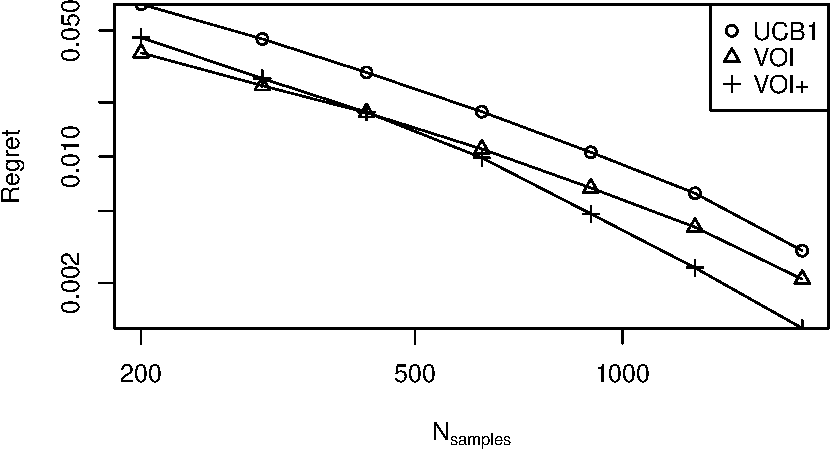
\includegraphics[scale=0.55]{mcts-flat.pdf}
\caption{Average regret of various policies as a function of the fixed number 
of samples in a 25-action Bernoulli sampling problem, over 10000 trials.}
\label{fig:random-instances}
\end{figure}

The sampling policies are compared on random Bernoulli
selection problem instances. Figure~\ref{fig:random-instances} shows results for
randomly-generated selection problems with 25 Bernoulli arms, where
the mean rewards of the arms are distributed uniformly in~$[0,1]$, 
for a range of sample budgets~$200..2000$, with multiplicative
step of~$2$, averaging over 10000 trials.  We compare UCB1 with the 
policies based on the bounds in
Equation~(\ref{eqn:mcts-bound-blnk-hoeffding}) (VOI) and
Equation~(\ref{eqn:mcts-erf-blinkered}) (VOI+).
UCB1 is always considerably worse than the VOI-aware sampling policies.


\section{Sampling in trees}
\label{sec:mcts-sampling-in-trees}

The previous section addressed the selection problem in the flat case.
Selection in trees is more complicated.  The goal of Monte-Carlo tree 
search \cite{Chaslot.montecarlo} at the root node 
is usually to select an action that appears to be the best based on outcomes
of \textit{search rollouts}.
But the goal of rollouts at non-root nodes
is different than at the root: here it is important to better approximate the
value of the node, so that selection at the root can be more informed. The exact analysis
of sampling at internal nodes is outside the scope of this study. At present we 
have no better proposal for internal nodes than to use UCT there.

We thus propose the following hybrid sampling scheme \cite{TolpinShimony.mcts}: 
	at the \emph{root node}, sample based on the VOI estimate;
	at \emph{non-root nodes}, sample using UCT.

Strictly speaking, even at the root node the stationarity assumptions
underlying our belief-state MDP for selection do not hold exactly. UCT
is an adaptive scheme, and therefore the values generated by sampling
at non-root nodes will typically cause values observed at children of
the root node to be non-stationary.  Nevertheless, sampling based on
VOI estimates computed as for stationary distributions works well in
practice. As illustrated by the empirical evaluation
(Section~\ref{sec:mcts-emp-go}), estimates based on
upper bounds on the VOI result in good sampling policies, which
exhibit performance comparable to the performance of some
state-of-the-art heuristic algorithms.


\subsection{Stopping criterion}
\label{sec:mcts-control-stopping-criterion}

When a sample has a known cost commensurable with the value of
information of a measurement, an upper bound on the intrinsic VOI can also
be used to stop the sampling if the intrinsic VOI of any arm
is less than the total cost of sampling $C$: $\max_i \Lambda_i \le C$.

The VOI estimates of Equations~(\ref{eqn:mcts-thm-be}) and~(\ref{eqn:mcts-bound-blnk-hoeffding})
include the remaining sample budget $N$ as a
factor, but given the cost of a single sample $c$, the cost of the
remaining samples accounted for in estimating the intrinsic VOI is
$C=cN$. $N$ can be dropped on both sides of the inequality,
giving a reasonable stopping criterion:
\begin{align}
\frac 1 N \Lambda_\alpha^b \le&\frac {\overline X_\beta^{n_\beta}}
  {n_\alpha}\Pr(\overline X_\alpha^{n_\alpha+N}\le\overline
  X_\beta^{n_\alpha})\le c\nonumber\\
\frac 1 N \max_i\Lambda_i^b\le &\max_i\frac {(1-\overline X_\alpha^{n_\alpha})} {n_i}\Pr(\overline
  X_i^{n_i+N}\ge\overline X_\alpha^{n_\alpha})\le c\nonumber\\
    &\forall i: i\ne\alpha
\label{eqn:mcts-stopping-blnk}
\end{align}
The empirical evaluation (Section~\ref{sec:mcts-emp-go})
confirms the viability of this stopping criterion and illustrates the
influence of the sample cost $c$ on the performance of
the sampling policy. When the sample cost $c$ is unknown, one can perform initial calibration experiments
to determine a reasonable value, as done in the following.

\subsection{Sample redistribution in trees}
\label{sec:mcts-control-redistribution}

The above hybrid approach assumes
that the information obtained from rollouts in the
current state is discarded after a real-world action is selected. In practice,
many successful Monte-Carlo tree search algorithms reuse rollouts
generated at earlier search states, if the sample traverses the
current search state during the rollout; thus, the value of information of a rollout is
determined not just by the influence on the choice of the action at
the current state, but also by its potential influence on the choice at future
search states.

One way to account for this reuse would be to incorporate the
`future' value of information into a VOI estimate. However, this 
approach requires a nontrivial extension of the theory of metareasoning for search.
Alternately, one can behave myopically with respect to the search tree depth:
\begin{enumerate}
\item Estimate VOI as though the information is discarded after each step,
\item Stop early if the VOI is below a certain threshold
   (see Section~\ref{sec:mcts-control-stopping-criterion}), and
\item Save the unused sample budget for search in future states, such that
   if the nominal budget is $N$, and the unused budget in the last state
   is $N_u$, the search budget in the next state will be $N+N_u$.
\end{enumerate}
In this approach, the cost $c$ of a sample in the current state is the
VOI of increasing the budget of a future state by one sample.  It is
unclear whether this cost can be accurately estimated, but supposing
a fixed value for a given problem type and algorithm implementation
would work. Indeed, the empirical evaluation (Section~\ref{sec:mcts-emp-go})
confirms that stopping and sample redistribution based on a learned
fixed cost  substantially improve the performance of the VOI-based
sampling policy in game tree search.


\subsection{Playing Go against UCT}
\label{sec:mcts-emp-go}

The hybrid policies were compared on the game Go, a search domain
in which UCT-based MCTS has been particularly successful
\cite{Gelly.mogo}. A modified version of Pachi \cite{Braudis.pachi}, a state of the art
Go program, was used for the experiments:
\begin{itemize}
\item The UCT engine of Pachi was extended with VOI-aware sampling
  policies at the first step. 
\item The stopping criterion for the VOI-aware policy was
  modified and based solely on the sample cost, specified as
  a constant parameter. The heuristic stopping criterion for the
  original UCT policy was left unchanged.
\item The time-allocation model based on the fixed number of samples
  was modified for \textit{both the original UCT policy and the VOI-aware
  policies} such that 
  \begin{itemize}
    \item Initially, the same number of samples is available to
      the agent at each step, independently of the number of pre-simulated
      games;  
    \item If samples were unused at the current step,
      they become available at the next step. 
  \end{itemize}
\end{itemize}
While the UCT engine is not the most powerful engine of Pachi, it is still a strong
player. On the other hand, additional features of more advanced
engines would obstruct the MCTS phenomena which are the subject of
the experiment. The source code is available from
\url{http://github.com/dtolpin/uct}.
\begin{figure}[h!]
\centering
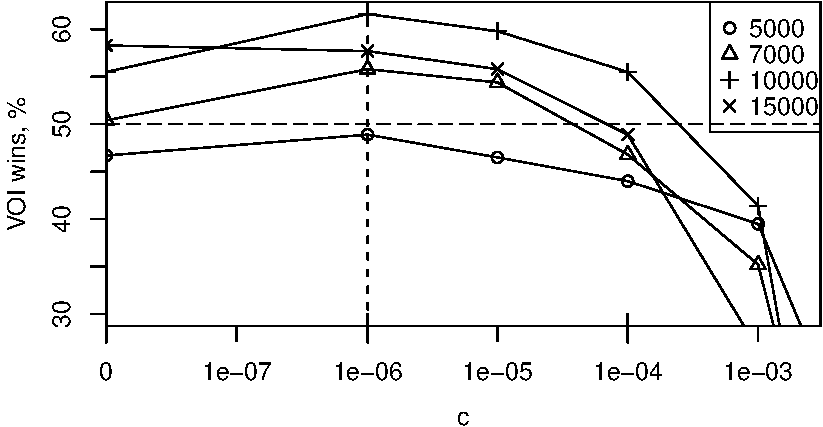
\includegraphics[scale=0.55]{mcts-uctvoi.pdf}
\caption{Winning rate of the VOI-aware policy in Go as a function of the cost $c$, for varying numbers of samples per ply.}
\label{fig:uctvoi}
\end{figure}
The engines were compared on the 9x9 board, for 5000, 7000, 1000, and
15000 samples (game simulations) per ply, each experiment repeated
1000 times. Figure~\ref{fig:uctvoi} depicts a calibration experiment,
showing the winning rate of the VOI-aware policy against UCT as a function of
the stopping threshold $c$ (if the maximum VOI of a sample is below
the threshold, the simulation is stopped, and a move is chosen). Each
curve in the figure corresponds to a certain number of samples per
ply.  For the stopping threshold of $10^{-6}$, the VOI-aware policy
is almost always better than UCT, and reaches the winning rate of
64\% for 10000 samples per ply.

\begin{figure}[h!]
\centering
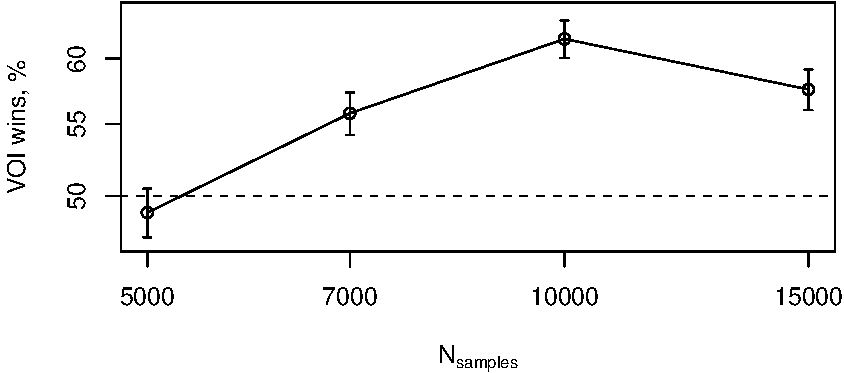
\includegraphics[scale=0.55]{mcts-voi-wins.pdf}
\caption{Winning rate of the VOI-aware policy in Go as a function of the number of samples, fixing cost $c=10^{-6}$.}
\label{fig:voi-wins}
\end{figure}

Figure~\ref{fig:voi-wins}
shows the winning rate of VOI against UCT $c=10^{-6}$. In agreement with the intuition
(Section~\ref{sec:mcts-control-redistribution}), VOI-based stopping and
sample redistribution is most influential for intermediate numbers of
samples per ply. When the maximum number of samples is too low, early
stopping would result in poorly selected moves. On the other hand,
when the maximum number of samples is sufficiently high, the VOI of
increasing the maximum number of samples in a future state is low.

Note that if we disallowed reuse of samples in both Pachi and
in our VOI-based scheme, the VOI based-scheme
win rate is even higher than shown in Figure~\ref{fig:voi-wins}. This is as expected,
as this setting (which is somewhat unfair to UCT-Pachi) is closer to
meeting the assumptions underlying the selection MDP.

\section{Conclusion and Further Research}

This work suggested a Monte-Carlo sampling policy in which sample
selection is based on upper bounds on the value of
information. Empirical evaluation showed that this policy outperforms
heuristic algorithms for pure exploration in MAB, as well as for MCTS.

MCTS still remains a largely unexplored field of
application of VOI-aware algorithms. More elaborate VOI estimates,
taking into consideration re-use of samples in future search states
should be considered. The policy introduced here differs from
the UCT algorithm only at the first step, where the VOI-aware
decisions are made. Consistent application of principles of rational
metareasoning at all steps of a rollout may further improve the
sampling.



\clearpage
\section{Towards Rational Deployment of Multiple Heuristics in A*}
\label{sec:cs-rla}

This study examines improvements to the \astar~algorithm when we have
several available admissible heuristics $h_1$, $h_2$, ... . Clearly, we can evaluate all
these heuristics, and use their {\em maximum} as an admissible
heuristic, a scheme we call \astarmax.  The problem with naive
maximization is that all the heuristics are computed for all the
generated nodes.  In order to reduce the time spent on heuristic
computations, Lazy $\astar$ (or \lazyastar, for short) evaluates the
heuristics one at a time, lazily.  When a node $n$ is generated,
\lazyastar~only computes one heuristic, $h_1(n)$, and adds $n$ to
\OPEN.  Only when $n$ re-emerges as the top of \OPEN~is another
heuristic, $h_2(n)$, evaluated; if this results in an increased
heuristic estimate, $n$ is re-inserted into \OPEN.  \lazyastar~is as
informative as \astarmax, but can significantly reduce search time, as
we will not need to compute $h_2$ for many nodes.

\lazyastar~reduces the search time, while maintaining the informativeness of \astarmax.
However, if the goal is reducing search time, it is sometimes better
to compute a fast heuristic on several nodes, rather than to compute a
slow but informative heuristic on only one node. We combine the ideas
of lazy heuristic evaluation and of trading off more node expansions
for less heuristic computation time, into a {\em new} variant of
\lazyastar~called {\em rational lazy} \astar~(\rationallazyastar).
\rationallazyastar~is based on rational metareasoning, and uses a
myopic {\em value-of-information} criterion to decide whether to
compute $h_2(n)$ or to bypass the computation of $h_2$ and expand $n$
immediately when $n$ re-emerges from \OPEN. \rationallazyastar~aims to
reduce search time, even at the expense of more node expansions than
\astarmax.

\section{Background and Related Work}

The \astar~algorithm \cite{ASTR68} is a best-first heuristic search
algorithm guided by the cost function $f(n)=g(n)+h(n)$.  If the
heuristic $h(n)$ is admissible (never overestimates the real cost to
the goal) then the set of nodes expanded by \astar~is both necessary
and sufficient to find the optimal path to the goal~\cite{ASTR85}.

Throughout this study we assume for clarity that we have two available
admissible heuristics, $h_1$ and $h_2$.
Unless stated otherwise, we assume that $h_1$ is faster to compute than $h_2$
but that $h_2$ is {\em weakly more informed}, i.e., $h_1(n) \leq h_2(n)$ for
the majority of the nodes $n$, although counter cases where $h_1(n) > h_2(n)$
are possible. We say that $h_2$ {\em dominates} $h_1$, if such counter cases do not
exist and $h_2(n) \geq h_1(n)$ for {\em all} nodes $n$.
We use $f_1(n)$ to denote $g(n)+h_1(n)$. Likewise, $f_2(n)$
denotes $g(n)+h_2(n)$, and $f_{max}(n)$ denotes $g(n) + \max(h_1(n),h_2(n))$.
We denote the cost of the optimal solution by $\optcost$. Additionally, we
denote the computation time of $h_1$ and of $h_2$ by $t_1$ and $t_2$,
respectively and denote the overhead of an {\em insert/pop} operation in
\OPEN~by $t_o$. Unless stated otherwise we assume that $t_2$ is much greater
than $t_1 + t_o$. 

\subsection{Selective MAX}

Based on the idea of of trading off more node expansions for less
heuristic computation time, \cite{domshlak-et-al:jair-2012} formulated
{\em selective max} (Sel-MAX), an online learning scheme which chooses
one heuristic to compute at each state. Sel-MAX chooses to compute the
more expensive heuristic $h_2$ for node $n$ when its classifier
predicts that $h_2(n) - h_1(n)$ is greater than some threshold, which
is a function of heuristic computation times and the average branching
factor.

\subsection{Lazy \astar}

The idea behind the \lazyastar~algorithm was briefly mentioned
by~\cite{zhang-bacchus:aaai-2012} in the context of the MAXSAT
heuristic for planning domains. \cite{Helmert.fdps} described
\emph{deferred evaluation} of heuristics in the context of the Fast
Downward Planning System. In deferred evaluation, the successors of
node $n$ are placed in the open list with the heuristic estimate of
$n$ and heuristically evaluated only when expanded.  The technique
bears a similarity to a special case of \lazyastar~where the first
heuristic always returns 0.

The pseudo-code for  \lazyastar~is depicted as Algorithm \ref{LAZYA}.
\lazyastar~mainly aims to reduce computations of $h_2$.
\begin{algorithm}[h]
\caption{Lazy \astar}
\begin{algorithmic}[1]
\Procedure{LAZY-\astar}{}
    \State Apply all heuristics to Start
    \State Insert Start into \OPEN
    \While{\OPEN~ not empty}
        \State $n$ $\gets$ best node from \OPEN
        \If{Goal(n)}
            \Return Trace(n)
        \EndIf
        \If{$h_2$ was not applied to $n$} \label{alg:rla-if-not-h2-beg}
            \State Apply $h_2$ to $n$
            State Insert $n$ into \OPEN
			\State {\bf continue} \Comment next node in OPEN
        \EndIf                           \label{alg:rla-if-not-h2-end}
        \ForAll{child $c$ of $n$}        \label{alg:rla-open-beg}
            \State Apply $h_1$ to $c$
            \State Insert $c$ into \OPEN
        \EndFor                          \label{alg:rla-open-end}
        \State Insert $n$ into \CLOSED
    \EndWhile  \\
    \Return FAILURE
\EndProcedure
\end{algorithmic}
\label{LAZYA}
\end{algorithm}
\lazyastar is very similar to \astar.
In fact, without lines~\ref{alg:rla-if-not-h2-beg}--\ref{alg:rla-if-not-h2-end}, \lazyastar~would be identical to
\astar~using the $h_1$ heuristic.
When a node $n$ is generated we only compute $h_1(n)$ and $n$ is added to
\OPEN ~(lines \ref{alg:rla-open-beg}--\ref{alg:rla-open-end}), without computing $h_2(n)$ yet.
When $n$ is first removed from \OPEN~(lines~\ref{alg:rla-if-not-h2-beg}--\ref{alg:rla-if-not-h2-end}), we compute $h_2(n)$ and
reinsert it into \OPEN, this time with $f_{max}(n)$.

It is easy to see that \lazyastar~is as informative as \astarmax, in
the sense that both \astarmax~and \lazyastar~expand a node $n$ only
if $f_{max}(n)$ is the best $f$-value in \textsc{Open}.  Therefore,
\lazyastar~and \astarmax~generate and expand and the same set of
nodes, up to differences caused by tie-breaking.

In its general form \astar~generates many nodes that it does not expand. These
nodes, called {\em surplus} nodes~\cite{Felner2012}, are in \OPEN~when we
expand the goal node with $f=\optcost$. All nodes in \OPEN~with $f>\optcost$ are
surely surplus but some nodes with $f=\optcost$ may also be surplus. The number
of surplus nodes in \OPEN can grow exponentially in the size of the domain, resulting in
significant costs.

\lazyastar~avoids $h_2$ computations for many of these surplus nodes. Consider
a node $n$ that is generated with $f_1(n) > \optcost$. This node is inserted
into \OPEN~but will never reach the top of \OPEN, as the goal node will be found
with $f=\optcost$. In fact, if \OPEN~breaks ties in favor of small $h$-values,
the goal node with $f=\optcost$ will be expanded as soon as it is generated and such
savings of $h_2$ will be obtained for some nodes with $f_1=\optcost$ too. We
refer to such nodes where we saved the computation of $h_2$ as {\em good} nodes. Other nodes,
those with $f_1(n) < \optcost$ (and some with $f_1(n) = \optcost$) are called
{\em regular nodes} as we apply both heuristics for them.

\section{Rational Lazy A*}

Using the principles of rational metareasoning (Section~\ref{sec:ratimeta}),
theoretically every computational operator (heuristic function evaluation, node
expansion, open list operation) should be treated as an action in a sequential
decision-making meta-level problem, and actions should be chosen so as to
achieve the minimal expected search time. However, the appropriate
general metareasoning problem is extremely hard to define precisely, and even harder
to solve optimally.

Therefore, we focus here on just one decision type, to be made in the
context of \lazyastar, when $n$ re-emerges from \OPEN~(Line 8).  We
have two options: {\bf (1)} Evaluate the second heuristic $h_2(n)$ and
add the node back to \OPEN~(lines~\ref{alg:rla-if-not-h2-beg}--\ref{alg:rla-if-not-h2-end}) like \lazyastar, or {\bf 2}
bypass the computation of $h_2(n)$ and expand $n$ right way~(lines~\ref{alg:rla-open-beg}--\ref{alg:rla-open-end}), thereby saving time by not computing $h_2$, at the risk of
additional expansions and evaluations of $h_1$.  A method which
attempts to optimally manage this trade-off, which we
call \textit{Rational Lazy A*} (\rationallazyastar), is presented
next.  In order to choose rationally we define a criterion based on
value of information (VOI) of evaluating $h_2(n)$ in this context.

The only addition of RLA* to LA* is the option to bypass $h_2$ computations~(lines~\ref{alg:rla-if-not-h2-beg}--\ref{alg:rla-if-not-h2-end}).
Suppose that we choose to compute $h_2$ --- this results in one of the
following outcomes:
\begin{enumerate}
\item $n$ is eventually expanded.
\item $n$ is re-inserted into \OPEN, and the goal is found without ever expanding $n$.
\end{enumerate}

Observe that computing $h_2$ can be beneficial only in outcome 2,
where potential time savings are due to pruning a search subtree at
the expense of the time $t_2(n)$. However, whether outcome 2 takes
place after a given state is not known to the algorithm until the goal
is found, and the algorithm must decide whether to evaluate $h_2$
according to what it \textit{believes to be} the probability of each
of the outcomes. The time wasted by being sub-optimal in deciding
whether to evaluate $h_2$ is called the {\em regret} of the decision.
We derive a \textit{rational policy} for deciding when to evaluate
$h_2$, under the following assumptions:
\begin{enumerate}
\item The decision is made \textit{myopically}: the algorithm continues to
  behave like \lazyastar~starting with the children of
  $n$.
\item $h_2$ is \textit{consistent}: if evaluating $h_2$ is benefitial
  on $n$, it is also benefitial on any successor of $n$.
\end{enumerate}
If \rationallazyastar~is indeed better than $\lazyastar$, the
first assumption results in an upper bound on the regret. The empirical
evaluation (Section~\ref{sec:rla-empirical}) covers also the cases
where $h_2$ is not consistent. Despite violation of the second assumption,
\rationallazyastar~still exhibits the best performance among
the compared algorithms.

If $h_2(n)$ is not helpful and we decide to compute it, the effort for evaluating
$h_2(n)$ turns out to be wasted. On the other hand, if $h_2(n)$ is
helpful but we decide to bypass it, we needlessly expand $n$. Due to
the myopic assumption, \rationallazyastar~would evaluate both $h_1$
and $h_2$ for all children of $n$. Due to consistency of $h_2$,
the children of $n$ will never be expanded.
\begin{table}[h!]
\begin{center}
\begin{tabular}{|l|c|c|}
\hline
               & Compute $h_2$ & Bypass $h_2$\\
\hline
$h_2$ helpful &   0            & $t_e+(b(n)-1)t_d$\\
\hline
$h_2$ not helpful & $t_d$      & 0 \\
\hline
\end{tabular}
\end{center}
\caption{Time losses in Rational Lazy A*}
\label{tbl:rla-rational-lazy-a-time}
\end{table}

Table~\ref{tbl:rla-rational-lazy-a-time}
summarizes the regret of each possible decision, for each possible future
outcome; each column in the table represents a decision, while each row
represents a future outcome.
In the table, $t_d$ is the to time compute $h_2$ and re-insert $n$ into
\OPEN~thus delaying the expansion of $n$, $t_e$ is the time to remove $n$ from \OPEN,
expand $n$, evaluate $h_1$ on each of the $b(n)$ (``local branching factor'')
children $\{n'\}$ of $n$, and insert $\{n'\}$ into the open list.
Computing $h_2$ needless ``wastes'' $t_d$ time.
Bypassing $h_2$ computation when $h_2$ would have been helpful ``wastes''
$t_e+b(n)t_d$ time, but because computing $h_2$ would have cost $t_d$, the
regret is $t_e+(b(n)-1)t_d$.

Let us denote the probability that $h_2$ is helpful by
$p_h$. The expected regret of computing $h_2$ is thus $(1-p_h) t_d$.
On other hand, the expected regret of bypassing $h_2$ is $p_h(
t_e+(b(n)-1)t_d)$. As we wish to minimize the expected regret, we should thus evaluate $h_2$ just when:
\begin{equation}
(1-p_h) t_d < p_h (t_e+(b(n)-1)t_d)
\end{equation}
or equivalently:
\begin{equation}
(1-b(n) p_h) t_d < p_h t_e
\end{equation}

If $p_h b(n) \ge 1$, then the expected regret is minimized by always
evaluating $h_2$, regardless of the values of $t_d$ and $t_e$.  In
these cases, RLA* cannot be expected to do better than \lazyastar.
For example, in the 15-puzzle and its variants, the effective
branching factor is $\approx 2$. Therefore, if $h_2$ is expected to be
helpful for more than half of the nodes $n$ on which
\lazyastar~evaluates $h_2(n)$, then one should simply use \lazyastar.

For $p_h b(n) < 1$,  the decision of whether to evaluate $h_2$
depends on the values of $t_d$ and $t_e$:
\begin{equation}
\mbox{\bf evaluate }h_2\mbox{ \bf if }t_d<\frac {p_h} {1-p_hb(n)} t_e
\label{eqn:rla-criterion-general}
\end{equation}
Let us analyze $t_d$ and $t_e$. Denote by
$t_c$ the time to generate the children of $n$. Then we have:
\begin{align}
t_d&=t_2+t_o\nonumber\\
t_e&=t_o + t_c+b (n) t_1 + b(n) t_o
\label{eqn:rla-t-del-exp-expanded}
\end{align}
By substituting
(\ref{eqn:rla-t-del-exp-expanded}) into (\ref{eqn:rla-criterion-general}), obtain: {\bf evaluate} $h_2$ {\bf if}:
\begin{equation}
{t_2+t_o}<\frac {p_h \left[{t_c} + b (n)t_1+(b(n)+1){t_o}\right]} {1-p_hb(n)}
\label{eqn:rla-criterion-expanded}
\end{equation}
The factor $\frac {p_h} {1-p_hb(n)}$ depends on the potentially unknown
probability $p_h$, making it difficult to reach the optimum decision.
However, if our goal is just to do better than \lazyastar, then it is safe to replace $p_h$ by an upper bound on $p_h$.

We now turn to implementation-specific estimation of the respective runtimes.
\OPEN~in \astar~is frequently implemented as a priority queue, and thus we have, approximately,
$t_o=\tau \log N_o$ for some $\tau$, when the size of \OPEN~is $N_o$.
Evaluating $h_1$ is cheap in many domains, as is the
case with the Manhattan Distance heuristic in discrete domains, $t_o$ is the most significant part of
$t_{e}$. In such cases,
rule (\ref{eqn:rla-criterion-expanded}) can be approximated as (\ref{eqn:rla-criterion-gamma}):
\begin{align}
  &\mbox{\bf evaluate }h_2\mbox{ \bf if } t_2 < \frac {\tau p_h} {1-p_hb(n)} (b(n)+1)\log N_o
\label{eqn:rla-criterion-gamma}
\end{align}
Rule (\ref{eqn:rla-criterion-gamma})
recommends to evaluate $h_2$ mostly at late stages of the search,
when the open list is large, and in nodes with a higher branching factor.

In other domains, such as planning, both $t_1$ and $t_2$ are
significantly greater than both $t_o$ and $t_c$, and terms
not involving $t_1$ or $t_2$ can be dropped from
(\ref{eqn:rla-criterion-expanded}), resulting in Rule (\ref{eqn:rla-criterion-beta}):
\begin{align}
  &\mbox{\bf evaluate }h_2\mbox{ \bf if } \frac{t_2}{t_1} < \frac {p_hb(n)} {1-p_hb(n)}
\label{eqn:rla-criterion-beta}
\end{align}
The right-hand side of (\ref{eqn:rla-criterion-beta}) grows with $b(n)$, and here it is beneficial to evaluate $h_2$
only for nodes with a sufficiently large branching factor. On rearranging equation \ref{eqn:rla-criterion-beta},
we get the criterion which we actually use for planning domains,
which is to evaluate $h_2$ only when:
\begin{equation}
b(n) > \frac{t_2}{t_1 p_h \left(1 + \frac{t_2}{t_1}\right)}
\label{eqn:rla-planning-rule}
\end{equation}

\section{Empirical Evaluation}
\label{sec:rla-empirical}

\subsection{Weighted 15-puzzle}

In the uniform-cost 15 puzzle, the open list contains only a few
different f-costs, and is frequently implemented using buckets,
violating the assumption of logarithmic time for which \rationallazyastar~is
beneficial. In order to better evaluate \rationallazyastar, we therefore use
the weighted 15-puzzle variant, where the cost of moving each tile is
equal to the number on the tile.  For consistency of comparison, we
used a subset of 36 problem instances out of the set of 100 15-puzzle
instances by~\cite{BFID85}, keeping the problems which could be solved
with 2Gb of RAM and 15 minutes timeout using the weighted Manhattan
distance heuristic (WMD) for $h_1$. As the second, expensive and informative,
$h_2$ heuristic for \lazyastar~and \rationallazyastar, we a heuristic
based on lookaheads~\cite{DBLP:conf/aaai/SternKFH10}. Given a bound
$d$ we applied a bounded depth-first search from a node $n$ and
backtracked when we reached leaf nodes $l$ for which $g(l)+WMD(l)>
g(n)+WMD(n)+d$. $f$-values from leaves were propagated to $n$.

\begin{table}
\parindent -0.5in
\begin{small}
\begin{tabular}{|c|| r r || r r r || r r r r r | } \hline
&\multicolumn{2}{|c||}{\astar}&\multicolumn{3}{c||}{\lazyastar}&\multicolumn{5}{c|}{\rationallazyastar}\\
\hline
lookahead & generated & time &  Good1 & $N_2$ & time & generated & Good1   & Good2  & $N_2$     & time \\ \hline
         6 & 889,930  & {\bf 0.601}  & 257,598 & 632,332 & 0.462   & 944,750 &  299,479 & 239,320 &  405,951   & 0.446  \\ \hline
         8 & 740,513  & 0.700  & 197,107 & 543,406 & {\bf 0.431}   & 892,216 &  233,370 & 303,655 &  260,823   & 0.402  \\ \hline
         10 & 612,010 & 0.929  & 145,687 & 466,327 & 0.474   & 859,220 &  278,431 & 445,846 &  134,943   & {\bf 0.378}  \\ \hline
         12 & 454,171 & 1.128  & 95,118  & 359,053 & 0.621   & 807,846 &  277,783 & 428,686 &  101,377   & 0.465  \\ \hline
\end{tabular}
\end{small}
\caption{Weighted 15 puzzle: comparison of $A^*_{\max}$, Lazy $A^*$, and Rational Lazy $A^*$}
\label{tbl:rla-rational-lazy-a-star}
\end{table}
Table~\ref{tbl:rla-rational-lazy-a-star} presents the results averaged
on all instances solved. The running times are reported relative
to the time of \astar~with WMD (with no lookahead), which generated
2012643 nodes (not reported in the table). The first 3 columns of Table
\ref{tbl:rla-rational-lazy-a-star} shows the results for \astar~with the
lookahead heuristic for different lookahead depths. The best time is
achieved for lookahead 6, (0.601 compared to \astar~with WMD). The fact
that the time does not continue to decrease with deeper lookaheads is
clearly due to the fact that although the resulting heuristic improves
as a function of lookahead depth (expanding and generating fewer nodes),
the increasing overheads of computing the heuristic eventually outweights
the computation time it saved by expanding fewer nodes.

The next 3 columns show the results for \lazyastar~ with WMD as $h_1$,
lookahead as $h_2$, for different lookahead depths
(\lazyastar~generates the same number of nodes as \astar).  The {\em
  Good1} column presents the number of nodes where \lazyastar saved
the computation of $h_2$ while the $N_2$ column presents the number of
nodes where $h_2$ was computed. $\approx 28\%$ of nodes were {\em
  Good1} and since $t_2$ was the most dominant time cost, most of this
saving is reflected in the timing results.  The best results are
achieved for lookahead 8, with a runtime of 0.431 compared to \astar~
with WMD.

The final columns show the results of \rationallazyastar, with the
values of $\tau$, $p_h$, $t_2$ calibrated for each lookahead depth using a
small subset of problem instances.  The {\em Good2} column counts the
number of times that \rationallazyastar~decided to bypass the $h_2$ computation and
expand the node right away. Observe that \rationallazyastar~outperforms \lazyastar,
which in turn outperforms standard A*, for all lookahead depths. The
lowest time with \rationallazyastar~(0.378 of \astar with WMD) and empirically best
$\tau$ was obtained for lookahead 10. That is achieved because the
more expensive $h_2$ heuristic is computed less often, reducing its
effective computational overhead, with little or no adverse effect in
the number of expanded nodes. Although LA* expanded fewer nodes,
\rationallazyastar~performed much fewer $h_2$ computations as can be seen in the table,
resulting in decreased overall runtimes for all lookahead depths.

The case of both $t_1$ and $t_2$ being significantly larger than $t_o$
and $t_c$ can also be modeled using the 15-puzzle domain by considering only the
time spent evaluating the heuristics. Table~\ref{tbl:rla-amax-la-rla-times}
presents the results of solving the Weighted 15-puzzle obtained on
the the set of 100 15-puzzle instances by~\cite{BFID85}, using the
combination of weighted Manhattan distance and linear
conflict \cite{hanssonmy.linconflict} heuristics. Rows $N_1$ and $N_2$ present the
average numbers of evaluations of $h_1$ and $h_2$, rows $T_1$ and
$T_2$ the average total times (per instance) spent evaluating each
of the heuristics.
\begin{table}[h!]
\begin{center}
\begin{tabular}{|l | c | c | c | } \hline
  &\astarmax&\lazyastar&\rationallazyastar\\ \hline 
$N_1$ & 1,482,271 & 1,482,271 & 1,521,163 \\ \hline
$T_1, sec$ & 0.979     & 0.979     & 1.026 \\ \hline
$N_2$ & 1,482,271 & 1,117,826 & 868,182 \\ \hline
$T_2, sec$ & 4.122     & 2.425     & 1.938 \\ \hline
$T_1+T_2, sec$ & 5.101 & 3.404    & 2.964 \\ \hline
\end{tabular}
\end{center}
\caption{Weighted 15 puzzle: comparison of heuristic computation times
in $A^*_{\max}$, Lazy $A^*$, and Rational Lazy $A^*$} 
\label{tbl:rla-amax-la-rla-times}
\end{table}
\astarmax~evaluates both $h_1$ and $h_2$ on both nodes and is obviously
the slowest. \lazyastar~evaluates $h_2$ selectively, spending 40\%
less time evaluating $h_2$ and 33\% less time
overall. \rationallazyastar, using Rule~(\ref{eqn:rla-planning-rule}),
spends 20\% less time than \lazyastar~evaluating $h_2$ \emph{at the
  expense} of spending 4\% more time evaluating $h_1$, and takes
12\% less time than \lazyastar~and 40\% less time than \astarmax~overall.

\subsection{Planning Domains}

\cite{TolpinEtAl.rla} presents results for comparing \rationallazyastar and
other algorithms on 42 planning domains. In these domains, time spent evaluating
heuristics constitutes approximately 90\% of the total search time,
hence applying rule~(\ref{eqn:rla-planning-rule}) is justified. 
\rationallazyastar~was compared to \lazyastar~and to \astar~using
each of the heuristics individually, as well as to the max-based
combination of the heuristics, and to the combination using selective-max
(Sel-MAX)~\cite{domshlak-et-al:jair-2012}. In the evaluation, 
\rationallazyastar~solved most problem instances in the shortest
total search time.
\begin{table}[h!]
\parindent -0.5in
\tiny{
\begin{tabular}{|l|r|r|r|r|r|r||r|r|r|r|r|r||r|r|r|r|r|r||r|r|}
\hline &
\multicolumn{6}{|c||}{Problems Solved } &
\multicolumn{6}{|c||}{Planning Time (seconds)} &
%\multicolumn{6}{|c||}{Expansions (623)} &
\multicolumn{2}{|c|}{GOOD } \\
\hline Domain &
$h_{LA}$ & lmcut & max & selmax & \lazyastar& \rationallazyastar &
$h_{LA}$ & lmcut & max & selmax & \lazyastar& \rationallazyastar &
%$h_1$ & $h_2$ & M & S & L& R &
\lazyastar& \rationallazyastar \\

\hline airport & 25 & 24 & 26 & 25 & \textbf{29} & \textbf{29} & \textbf{0.29} & 0.57 & 0.5 & 0.33bb & 0.38 & 0.38 & 0.48 & 0.67 \\
barman-opt11 & \textbf{4} & 0 & 0 & 0 & 0 & 3 & N/A & N/A & N/A & N/A & N/A & N/A & N/A & N/A \\
blocks & 26 & 27 & 27 & 27 & \textbf{28} & \textbf{28} & 1.0 & \textbf{0.65} & 0.73 & 0.81 & 0.67 & 0.67 & 0.19 & 0.21 \\
depot & \textbf{7} & 6 & 5 & 5 & 6 & 6 & \textbf{2.27} & 2.69 & 3.17 & 3.14 & 2.73 & 2.75 & 0.06 & 0.06 \\
driverlog & 10 & \textbf{12} & \textbf{12} & \textbf{12} & \textbf{12} & \textbf{12} & 2.65 & \textbf{0.29} & 0.33 & 0.36 & 0.3 & 0.31 & 0.09 & 0.09 \\
elevators-opt08 & 12 & \textbf{18} & 17 & 17 & 17 & 17 & 14.14 & 4.21 & 4.84 & 4.85 & \textbf{3.56} & 3.64 & 0.27 & 0.27 \\
elevators-opt11 & 10 & \textbf{14} & \textbf{14} & \textbf{14} & \textbf{14} & \textbf{14} & 26.97 & 8.03 & 9.28 & 9.28 & \textbf{6.64} & 6.78 & 0.28 & 0.28 \\
floortile-opt11 & 2 & \textbf{6} & \textbf{6} & \textbf{6} & \textbf{6} & \textbf{6} & 8.52 & \textbf{0.44} & 0.6 & 0.58 & 0.5 & 0.52 & 0.02 & 0.02 \\
freecell & \textbf{54} & 10 & 36 & 51 & 41 & 41 & \textbf{0.16} & 7.34 & 0.22 & 0.24 & 0.18 & 0.18 & 0.86 & 0.86 \\
grid & \textbf{2} & \textbf{2} & 1 & \textbf{2} & \textbf{2} & \textbf{2} & \textbf{0.1} & 0.16 & 0.18 & 0.34 & 0.15 & 0.15 & 0.17 & 0.17 \\
gripper & \textbf{7} & 6 & 6 & 6 & 6 & 6 & \textbf{0.84} & 1.53 & 2.24 & 2.2 & 1.78 & 1.25 & 0.01 & 0.4 \\
logistics00 & \textbf{20} & 17 & 16 & \textbf{20} & 19 & 19 & \textbf{0.23} & 0.57 & 0.68 & 0.27 & 0.47 & 0.47 & 0.51 & 0.51 \\
logistics98 & 3 & \textbf{6} & \textbf{6} & \textbf{6} & \textbf{6} & \textbf{6} & 0.72 & \textbf{0.1} & 0.1 & 0.11 & \textbf{0.1} & \textbf{0.1} & 0.07 & 0.07 \\
miconic & \textbf{141} & 140 & 140 & \textbf{141} & \textbf{141} & \textbf{141} & \textbf{0.13} & 0.55 & 0.58 & 0.57 & 0.16 & 0.16 & 0.87 & 0.88 \\
mprime & 16 & 20 & 20 & 20 & \textbf{21} & 20 & 1.27 & 0.5 & 0.51 & 0.5 & \textbf{0.44} & 0.45 & 0.25 & 0.25 \\
mystery & 13 & \textbf{15} & \textbf{15} & \textbf{15} & \textbf{15} & \textbf{15} & 0.71 & \textbf{0.35} & 0.38 & 0.43 & 0.36 & 0.37 & 0.3 & 0.3 \\
nomystery-opt11 & \textbf{18} & 14 & 16 & \textbf{18} & \textbf{18} & \textbf{18} & \textbf{0.18} & 1.29 & 0.58 & 0.25 & 0.33 & 0.33 & 0.72 & 0.72 \\
openstacks-opt08 & 15 & \textbf{16} & 14 & 15 & \textbf{16} & \textbf{16} & 2.88 & \textbf{1.68} & 3.89 & 3.03 & 2.62 & 2.64 & 0.44 & 0.45 \\
openstacks-opt11 & 10 & \textbf{11} & 9 & 10 & \textbf{11} & \textbf{11} & 13.59 & \textbf{6.96} & 19.8 & 14.44 & 12.03 & 12.06 & 0.43 & 0.43 \\
parcprinter-08 & 14 & \textbf{18} & \textbf{18} & \textbf{18} & \textbf{18} & \textbf{18} & 0.92 & \textbf{0.36} & 0.37 & 0.38 & 0.37 & 0.37 & 0.17 & 0.26 \\
parcprinter-opt11 & 10 & \textbf{13} & \textbf{13} & \textbf{13} & \textbf{13} & \textbf{13} & 2.24 & \textbf{0.56} & 0.6 & 0.61 & 0.58 & 0.59 & 0.14 & 0.17 \\
parking-opt11 & 1 & 1 & 1 & \textbf{3} & 2 & 2 & 9.74 & 22.13 & 17.85 & 7.11 & \textbf{6.33} & 6.43 & 0.64 & 0.64 \\
pathways & 4 & \textbf{5} & \textbf{5} & \textbf{5} & \textbf{5} & \textbf{5} & 0.5 & \textbf{0.1} & \textbf{0.1} & \textbf{0.1} & \textbf{0.1} & \textbf{0.1} & 0.1 & 0.12 \\
pegsol-08 & \textbf{27} & \textbf{27} & \textbf{27} & \textbf{27} & \textbf{27} & \textbf{27} & 1.01 & \textbf{0.84} & 1.2 & 1.1 & 1.06 & 0.95 & 0.04 & 0.42 \\
pegsol-opt11 & \textbf{17} & \textbf{17} & \textbf{17} & \textbf{17} & \textbf{17} & \textbf{17} & 4.91 & \textbf{3.63} & 5.85 & 5.15 & 4.87 & 4.22 & 0.04 & 0.38 \\
pipesworld-notankage & \textbf{16} & 15 & 15 & \textbf{16} & 15 & 15 & \textbf{0.5} & 1.48 & 1.12 & 0.85 & 0.9 & 0.91 & 0.42 & 0.42 \\
pipesworld-tankage & \textbf{11} & 8 & 9 & 9 & 9 & 9 & \textbf{0.36} & 2.24 & 1.02 & 0.47 & 0.69 & 0.71 & 0.62 & 0.62 \\
psr-small & \textbf{49} & 48 & 48 & \textbf{49} & 48 & 48 & \textbf{0.15} & 0.2 & 0.21 & 0.19 & 0.19 & 0.18 & 0.17 & 0.49 \\
rovers & 6 & \textbf{7} & \textbf{7} & \textbf{7} & \textbf{7} & \textbf{7} & 0.74 & \textbf{0.41} & 0.45 & 0.45 & 0.41 & 0.42 & 0.47 & 0.47 \\
scanalyzer-08 & 6 & \textbf{13} & \textbf{13} & \textbf{13} & \textbf{13} & \textbf{13} & 0.37 & \textbf{0.25} & 0.27 & 0.27 & 0.26 & 0.26 & 0.06 & 0.06 \\
scanalyzer-opt11 & 3 & \textbf{10} & \textbf{10} & \textbf{10} & \textbf{10} & \textbf{10} & \textbf{0.59} & 0.64 & 0.75 & 0.73 & 0.67 & 0.68 & 0.05 & 0.05 \\
sokoban-opt08 & 23 & 25 & 25 & 24 & 26 & \textbf{27} & 3.94 & 1.76 & 2.19 & 2.96 & 1.9 & \textbf{1.32} & 0.04 & 0.4 \\
sokoban-opt11 & \textbf{19} & \textbf{19} & \textbf{19} & 18 & \textbf{19} & \textbf{19} & 7.26 & 2.83 & 3.66 & 5.19 & 3.1 & \textbf{2.02} & 0.03 & 0.46 \\
storage & 14 & \textbf{15} & 14 & 14 & \textbf{15} & \textbf{15} & \textbf{0.36} & 0.44 & 0.49 & 0.45 & 0.44 & 0.42 & 0.21 & 0.28 \\
tidybot-opt11 & \textbf{14} & 12 & 12 & 12 & 12 & 12 & \textbf{3.03} & 16.32 & 17.55 & 9.35 & 15.67 & 15.02 & 0.11 & 0.18 \\
tpp & \textbf{6} & \textbf{6} & \textbf{6} & \textbf{6} & \textbf{6} & \textbf{6} & 0.39 & \textbf{0.22} & 0.23 & 0.23 & 0.22 & 0.22 & 0.32 & 0.4 \\
transport-opt08 & \textbf{11} & \textbf{11} & \textbf{11} & \textbf{11} & \textbf{11} & \textbf{11} & 1.45 & \textbf{1.24} & 1.41 & 1.54 & 1.25 & 1.26 & 0.04 & 0.04 \\
transport-opt11 & \textbf{6} & \textbf{6} & \textbf{6} & \textbf{6} & \textbf{6} & \textbf{6} & 12.46 & \textbf{8.5} & 10.38 & 11.13 & 8.56 & 8.61 & 0.0 & 0.0 \\
trucks & 7 & \textbf{9} & \textbf{9} & \textbf{9} & \textbf{9} & \textbf{9} & 4.49 & \textbf{1.34} & 1.52 & 1.44 & 1.41 & 1.42 & 0.07 & 0.07 \\
visitall-opt11 & 12 & 10 & \textbf{13} & 12 & \textbf{13} & \textbf{13} & 0.2 & 0.34 & 0.19 & \textbf{0.18} & 0.18 & 0.18 & 0.38 & 0.38 \\
woodworking-opt08 & 12 & \textbf{16} & \textbf{16} & \textbf{16} & \textbf{16} & \textbf{16} & 1.08 & 0.71 & 0.75 & 0.75 & \textbf{0.66} & 0.67 & 0.56 & 0.56 \\
woodworking-opt11 & 7 & \textbf{11} & \textbf{11} & \textbf{11} & \textbf{11} & \textbf{11} & 5.7 & 2.86 & 3.15 & 3.01 & \textbf{2.55} & 2.58 & 0.52 & 0.52 \\
zenotravel & 8 & \textbf{11} & \textbf{11} & \textbf{11} & \textbf{11} & \textbf{11} & 0.38 & \textbf{0.14} & 0.14 & 0.14 & 0.14 & 0.14 & 0.17 & 0.19 \\
\hline
OVERALL & 698 & 697 & 722 & 747 & 747 & \textbf{750} & 1.18 & 0.98 & 0.98 & 0.89 & 0.79 & \textbf{0.77} & 0.27 & 0.34 \\
\hline
\end{tabular}
}
\begin{small}
\caption{\label{tbl:rla-planning} Planning Domains --- Number of Problems
Solved, Total Planning Time, and Fraction of Good Nodes}
\end{small}
\end{table}

Table~\ref{tbl:rla-planning} depicts the experimental results
(provided by Erez Karpas). \lazyastar~and \rationallazyastar~were
implemented on top of the Fast Downward
planning system \cite{helmert:jair-2006}, and two state
of the art heuristics were used: the admissible landmarks heuristic $h_{LA}$ (used as $h_1$)
\cite{karpas-domshlak:ijcai-2009}, and the landmark cut heuristic $h_{LMCUT}$
\cite{helmert-domshlak:icaps-2009} (used as $h_2$).
On average, $h_{LMCUT}$ computation is 8.36 times more expensive than $h_{LA}$
computation.

The leftmost part of the table shows the number of solved problems in each
domain. As the table demonstrates, \rationallazyastar~solves the most problems,
and \lazyastar~solves the same number of problems as Sel-MAX. Thus, both
\lazyastar~and \rationallazyastar~are state-of-the-art in cost-optimal planning.
Looking more closely at the results, note that Sel-MAX
solves 10 more problems than \lazyastar~and \rationallazyastar~in the freecell
domain. Freecell is one of only three domains in which $h_{LA}$ is more
informed than $h_{LMCUT}$ ~(the other two are nomystery-opt11 and
visitall-opt11), violating the basic assumptions behind 
\lazyastar~ that $h_2$ is more informed than $h_1$. If
we ignore these domains, both \lazyastar~and \rationallazyastar~solve more
problems than Sel-MAX.

The middle part of the Table~\ref{tbl:rla-planning} shows the geometric mean of
planning time in each domain, over the commonly solved problems (i.e., those
that were solved by all 6 methods). \rationallazyastar~is the fastest overall,
with \lazyastar~second. It is important to note that both \lazyastar~and
\rationallazyastar~are very robust, and even in cases where they are not the
best they are never too far from the best. For example, consider the {\em
miconic} domain. Here,  $h_{LA}$ is very informative and thus the variant that
only computed $h_{LA}$ is the best choice (but a bad choice overall). Observe
that both  \lazyastar~and \rationallazyastar~saved 86\% of $h_{LMCUT}$
computations, and were very close to the best algorithm in this extreme case.
In contrast, the other algorithms that consider both heuristics (max and
Sel-MAX) performed very poorly here (more than three times slower).

The rightmost part of Table~\ref{tbl:rla-planning} shows the average
fraction of nodes for which \lazyastar~ and \rationallazyastar~did not evaluate
the more expensive heuristic, $h_{LMCUT}$, over the problems solved by both
these methods.
This is shown in the {\em good} columns. Our first observation is that this
fraction varies between different domains, indicating why \lazyastar~works well
in some domains, but not in others. Additionally, we can see that in domains
where there is a difference in this number between \lazyastar~and
\rationallazyastar, \rationallazyastar~usually performs better in terms of
time. This indicates that when \rationallazyastar~decides to skip the
computation of the expensive heuristic, it is usually the right
decision. 

\begin{table}[h!]
\begin{center}
\begin{small}
\begin{tabular}{|l|r|r|}
\hline
&  Expanded & Generated\\
\hline
$h_{LA}$     & 183,320,267 & 1,184,443,684\\
lmcut    & 23,797,219 & 114,315,382\\
\astarmax          & 22,774,804 & 108,132,460\\
selmax          & 54,557,689 & 193,980,693\\
\hline
$\lazyastar$  & 22,790,804 & 108,201,244\\
$\rationallazyastar$   & 25,742,262 & 110,935,698\\
\hline
\end{tabular}
\end{small}
\end{center}
\caption{\label{tbl:rla-planning-states} Total Number of Expanded and Generated States}
\end{table}

Table~\ref{tbl:rla-planning-states} shows the total number of expanded and generated
states over all commonly solved problems. \lazyastar~is indeed as informative
as \astarmax~(the small difference is caused by tie-breaking), while
\rationallazyastar~is a little less informed and expands slightly more nodes.
However, \rationallazyastar~is much more informative than its ``intelligent''
competitor --- Sel-MAX, as these are the only two algorithms in our set
which selectively omit some heuristic computations.
\rationallazyastar~generated almost half of the nodes compared to
Sel-MAX, suggesting that its decisions are better. 

\section{Conclusion and Further Research}

We discussed a scheme for decreasing heuristic evaluation
times in \lazyastar. Compared to \lazyastar, \rationallazyastar~allows
additional cuts in $h_2$ evaluations, at the expense of being less
informed. However, due to a rational trade-off, this
allows for an additional speedup, and \rationallazyastar~achieves the
best overall performance in our domains.

In addition, \rationallazyastar~is simpler to implement than its direct
competitor, selective max, but its decision can be more informed.  When
\rationallazyastar~has to decide whether to compute $h_2$ for some node
$n$, it already {\em knows} that $f_1(n) \leq \optcost$.  By contrast,
although selective max uses a much more complicated decision rule, it
chooses which heuristic to compute when $n$ is first generated, and does
not know whether $h_1$ will be informative enough to prune $n$.
\rationallazyastar~outperforms selective max in our planning experiments.

There are numerous other ways to use rational metareasoning to
improve~\astar, starting from generalizing \rationallazyastar~to
handle more than two heuristics, to using the meta-level to control
decisions in other variants of \astar, such as \idastar. All these potential extensions
provide fruitful ground for further research.


\chapter {Summary and Contribution}
\label{ch:summary}
The thesis comprises two major topics:
\begin {enumerate}
\item Rational computation of value of information (Chapter~\ref{ch:raticomp}).
\item Case studies of application of rational metareasoning to
  selection and application of heuristic computations (Chapter~\ref{ch:case-studies}).
\end {enumerate}

The first topic addressed cases in which estimating the value
of information of a computational action is expensive, as well as
cases of too many computational actions, such that although
estimating the value of information of a single action is cheap,
estimating the value of information of all actions at each step of the
algorithm is expensive. The research, published in
\cite{TolpinShimony.raticomp}, resulted in an improvement to a widely
used class of VOI-based optimization algorithms that allows to decrease the
computation time while only slightly affecting the reward. Theoretical
analysis of the proposed approach to rational computation of the
value of information was supported by empirical evaluation of several
combinations of algorithms and search problems.

The second topic considered several search problems and improved some
well-known algorithms for solving the problems using the rational
metareasoning approach:
\begin {itemize}
\item Adaptive deployment of value-ordering heuristics in constraint
  satisfaction problems (Section~\ref{sec:cs-csp}) \cite{TolpinShimony.csp};
\item Monte Carlo tree search based on simple regret
  (Section~\ref{sec:cs-mcts}) \cite{TolpinShimony.mcts,HayRussellTolpinShimony.selecting};
\item Decreasing heuristic evaluation time in a variant of A*
  (Section~\ref{sec:cs-rla}) \cite{TolpinEtAl.rla}. 
\end {itemize}
In addition to the algorithm improvements, the studies demonstrated a
number of common rational metareasoning techniques which can be 
extended to other problem types. In particular,
\begin{itemize}
\item Section~\ref{sec:cs-mcts}, ``VOI-aware Monte-Carlo tree search''
provided distribution-independent upper bounds for semi-myopic VOI
estimates in Monte-Carlo sampling.
\item Section~\ref{sec:cs-rla}, ``Towards rational deployment of Multiple
Heuristics in A*'', introduced a novel area of application of rational
metareasoning---optimal search in optimization problems.
\end{itemize}

As a whole, the research advanced the use of rational
metareasoning in problem-solving search algorithms. Applications of
rational metareasoning in the case studies serve as examples
to help researchers employ the methodology in solutions for other
problems. Advances in rational computation and estimation of VOI increase
performance and applicability of existing and new search algorithms
and alleviate dependence of algorithm performance on manual
fine-tuning.

The field of rational metareasoning still poses serious
challenges. An important yet unanswered question is the extent
to which algorithm performance can be improved due to employment of
the metareasoning approach. In the case studies presented in the thesis,
the improvements, while approached the theoretical limits of each
particular algorithm variant, were moderate. It is still not clearly
understood \textbf{whether a dramatic breakthrough in performance is possible}
if more elaborated models of utility and information are used, or the 
limitations are immanent to the approach itself. Another interesting
field of research is rational metareasoning where \textbf{action costs and
state utilities are not commensurable}. Instead of mapping between
different measures, as suggested in Chapter~\ref{ch:raticomp}, a
more general combination function should probably be used for best
results. Ways of choosing or deriving such a function still remain
to be discovered.


\bibliographystyle{alpha}
\bibliography{refs}

\end{document}
